% Springer Nature journal article template
% Version 3.1, December 2024

\documentclass[pdflatex,sn-mathphys-num]{sn-jnl}

\usepackage{graphicx}
\usepackage{multirow}
\usepackage{amsmath,amssymb,amsfonts}
\usepackage{amsthm}
\usepackage{mathrsfs}
\usepackage[title]{appendix}
\usepackage{xcolor}
\usepackage{textcomp}
\usepackage{manyfoot}
\usepackage{booktabs}
\usepackage{algorithm}
\usepackage{algorithmicx}
\usepackage{algpseudocode}
\usepackage{listings}

\raggedbottom

\begin{document}

\title[Controlled evaluation of QUARTS]{QUARTS for Probabilistic Traffic Forecasting: A Controlled Evaluation of Quantum and Classical Residual Calibration}

\author*[1]{\fnm{Shishir Singh} \sur{Chauhan}}\email{shishir.chauhan@jaipur.manipal.edu}

\affil*[1]{\orgdiv{Department of Computer Science and Engineering},
\orgname{Manipal University Jaipur},
\orgaddress{\street{Jaipur-Ajmer Expressway}, \city{Jaipur},
\postcode{303007}, \state{Rajasthan}, \country{India}}}

\abstract{Quantum machine learning has been proposed for traffic forecasting, yet evidence from network traffic settings remains limited. We present QUARTS, a Quantum Uncertainty Aware Residual Traffic System, to test whether an entangled variational quantum circuit improves point forecasts or predictive intervals under identical experimental conditions. Experiments used METR-LA, PEMS-BAY, PeMSD4, and PeMSD8 with matched separable quantum, Fourier, multilayer perceptron, and unchanged backbone controls. Across five confirmatory seeds, entangled QUARTS obtained mean absolute errors of 3.897 on METR-LA and 2.030 on PEMS-BAY, which were 32.99\% and 31.84\% above STAEformer. Differences from the separable quantum and Fourier heads remained below 0.40\%, providing no evidence that entanglement produced a predictive gain. A classical Fourier regime aware calibrator reduced weighted interval score by 14.58\% relative to constant intervals and by 0.68\% relative to a multilayer perceptron in the initial prospective PeMSD4 run. Across five independently trained backbones, however, the mean Fourier minus multilayer perceptron difference was $-0.0308$ with a dependence aware $95\%$ interval of $[-0.1336,0.0767]$ and only three directional wins. A conformal quantile variant failed its PeMSD8 validation gate, so the test split remained untouched. The results show that strong forecasting backbones, matched nonlinear controls, and explicit validation gates are necessary for credible assessment of quantum traffic models.}

\keywords{traffic forecasting, quantum machine learning, variational quantum circuits, probabilistic forecasting, uncertainty calibration, conformal prediction}

\maketitle

\section{Introduction}\label{sec:introduction}

Traffic forecasts support network management, traveller information, congestion mitigation, and operational planning. Their practical value depends on two related properties. The central estimate should remain accurate over several future horizons, and the accompanying uncertainty should indicate when that estimate is less dependable. Both properties are difficult to obtain because traffic observations are coupled through a road network, change with recurring temporal regimes, and respond to incidents, missing measurements, and other disturbances. Reviews of the field therefore identify spatial dependence, temporal nonstationarity, transfer between networks, and trustworthy uncertainty as continuing problems rather than settled implementation details \cite{lana2018road,tedjopurnomo2022survey}.

Classical traffic forecasting has advanced rapidly on public sensor benchmarks. Diffusion convolution introduced directed graph propagation into recurrent forecasting \cite{li2018dcrnn}. Spatial and temporal graph convolution, adaptive adjacency learning, attention, and node specific embeddings subsequently improved the representation of network structure and periodic behaviour \cite{yu2018stgcn,wu2019graphwavenet,bai2020agcrn,guo2019astgcn,zheng2020gman}. More recent work shows that much of the predictive gain can arise from a suitable representation rather than an increasingly elaborate forecasting block. STID uses spatial and temporal identity information as a compact baseline \cite{shao2022stid}, while STAEformer combines adaptive spatial and temporal embeddings with a standard Transformer and reports strong results on common benchmarks \cite{liu2023staeformer}. These developments make a weak classical comparator unsuitable for assessing a quantum model.

Probabilistic forecasting adds a second requirement. A model can obtain a reasonable mean absolute error while producing intervals that are too narrow, too wide, or unstable under a change of traffic regime. Proper scoring rules provide a principled way to evaluate predictive distributions \cite{gneiting2007scoring}. The weighted interval score combines interval sharpness with penalties for observations outside the reported bounds and is suitable when several central intervals are available \cite{bracher2021wis}. Conformal prediction offers a complementary route to empirical coverage without requiring a fully specified conditional distribution \cite{angelopoulos2023conformal}. Conformalized quantile regression can adapt interval width to heterogeneous residual variance \cite{romano2019cqr}, although sequential traffic observations do not automatically satisfy the exchangeability assumptions used by standard conformal arguments. Methods developed for dynamic time series illustrate both the promise and the care needed in this setting \cite{xu2021enbpi}.

Quantum machine learning provides trainable feature maps and variational circuits that can be coupled to classical networks \cite{biamonte2017qml,cerezo2021vqa}. Data reuploading repeatedly encodes classical features and can generate rich nonlinear functions with a small number of qubits \cite{perezsalinas2020reuploading}. The resulting function class has a Fourier interpretation that depends on the encoding and observable \cite{schuld2021encoding}. This interpretation creates a demanding attribution problem. If a variational quantum circuit improves a forecast, the comparison must establish whether the gain comes from entanglement, from a periodic nonlinear basis that a classical Fourier layer can reproduce, or simply from adding trainable parameters. Broad quantum machine learning benchmarks have found that classical methods often remain stronger and that removing entanglement can leave performance unchanged or improve it on small learning tasks \cite{bowles2024benchmark}.

Transportation research has begun to examine quantum optimization, sensing, and prediction \cite{usdot2024quantum,mohammed2025annealingreview}. Direct traffic forecasting evidence is still limited. Schetakis et al.\ studied data reuploading quantum neural networks on a single urban detector and identified multiple input, multiple output, and transfer settings as important extensions \cite{schetakis2025trafficqnn}. Rajagopal et al.\ reported a quantum inspired graph formulation for traffic flow prediction \cite{rajagopal2025mthqgnn}. These studies motivate further investigation, but they do not resolve whether an executable entangled circuit contributes beyond matched classical nonlinear controls on standard network wide forecasting tasks.

This study addresses that question through QUARTS, the Quantum Uncertainty Aware Residual Traffic System. A classical forecasting backbone produces a base forecast and local latent state. A shared calibration head then estimates a point correction, an uncertainty scale, or interval radii. The head can be an entangled variational quantum circuit, a circuit with the entanglers removed, a classical Fourier module, a multilayer perceptron, or no learned calibrator. Every learned head receives the same local information and is evaluated under a common split, optimization budget, and metric definition. Later variants freeze STAEformer so that calibration cannot be mistaken for a stronger forecasting backbone.

The investigation is organized around four questions. First, does the entangled head improve point forecasting over the unchanged backbone and STAEformer? Second, does it outperform separable quantum, Fourier, and multilayer perceptron controls? Third, can regime aware residual calibration improve interval quality while maintaining nominal coverage? Fourth, do observed gains survive independent backbone initialization and a new dataset? These questions are evaluated with five confirmatory seeds on METR-LA and PEMS-BAY, prospective testing on PeMSD4, and a validation only transfer study on PeMSD8.

The study makes four contributions. First, it provides a controlled architecture that isolates the function of a small shared quantum calibrator from the network scale forecasting backbone. Second, it evaluates entanglement against a separable circuit and a Fourier control that directly reflects the known spectral structure of data reuploading models. Third, it links point accuracy, interval quality, calibration, computation time, circuit sensitivity, missing input robustness, and paired statistical analysis in one traceable protocol. Fourth, it reports the complete sequence of favourable, negative, and inconclusive findings. The confirmatory study does not support a quantum advantage. A classical Fourier regime calibrator shows a small prospective interval score improvement, but the expanded five backbone analysis contains two sign reversals and a confidence interval that crosses zero. The resulting contribution is therefore an evidence bounded account of what residual calibration achieved, where it failed, and why entanglement cannot be credited for the observed behaviour.

\section{Related work}\label{sec:related}

\subsection{Network traffic forecasting}\label{subsec:classical}

Traffic forecasting methods have moved from recurrent models with fixed spatial structure toward architectures that learn interactions jointly from data. DCRNN represents directed traffic propagation as diffusion on a graph \cite{li2018dcrnn}, while STGCN uses graph and temporal convolutions without recurrent units \cite{yu2018stgcn}. Graph WaveNet and AGCRN learn adaptive relations that can supplement or replace a prescribed road graph \cite{wu2019graphwavenet,bai2020agcrn}. ASTGCN and GMAN use attention to distinguish relevant locations and times \cite{guo2019astgcn,zheng2020gman}. MTGNN extends graph learning to general multivariate time series \cite{wu2020mtgnn}. PDFormer introduces propagation delay awareness, which is particularly relevant when congestion reaches nearby sensors at different times \cite{jiang2023pdformer}.

Recent results also question whether architectural complexity alone explains progress. STID obtains competitive accuracy through spatial and temporal identity embeddings \cite{shao2022stid}. STAEformer similarly uses adaptive embeddings to supply a Transformer with traffic specific context \cite{liu2023staeformer}. QUARTS therefore treats a strong backbone as a necessary comparator. The study does not claim that a small quantum head can replace graph scale representation learning. It asks the narrower question of whether such a head adds useful local residual structure after the backbone has formed its representation.

\subsection{Probabilistic forecasting and calibration}\label{subsec:probabilistic}

Probabilistic forecasting evaluates a distribution or a set of intervals rather than a single trajectory. DeepAR demonstrated how a shared autoregressive model can learn probabilistic forecasts across many related series \cite{salinas2020deepar}. Proper scoring rules discourage a forecaster from improving apparent coverage merely by widening every interval \cite{gneiting2007scoring}. The weighted interval score is especially useful when evaluation data contain a finite set of central intervals \cite{bracher2021wis}.

Conformal prediction separates the fitted predictor from a calibration step and offers finite sample marginal coverage under exchangeability \cite{angelopoulos2023conformal}. Conformalized quantile regression retains feature dependent interval width and then corrects residual miscoverage \cite{romano2019cqr}. Time ordered traffic data complicate the usual guarantee because adjacent observations are dependent and their distribution may drift. EnbPI addresses related difficulties with sequential residual updates \cite{xu2021enbpi}. In this study, conformal calibration is used as an empirical procedure on chronological validation data. Coverage is reported, and no claim of distribution free conditional coverage is made.

\subsection{Quantum learning and matched controls}\label{subsec:qml}

Variational quantum models commonly combine a classical input map, trainable quantum gates, measurement, and a classical readout \cite{biamonte2017qml,cerezo2021vqa}. Quantum feature maps can represent nonlinear similarities in a Hilbert space \cite{havlicek2019feature}, and data reuploading increases the expressiveness of small circuits \cite{perezsalinas2020reuploading}. Their representational power can exceed that of some similarly sized classical networks in selected settings \cite{abbas2021power}. However, expressibility is not equivalent to useful generalization. Highly expressive circuits may be difficult to train \cite{sim2019expressibility}; gradients can vanish with circuit size or unsuitable initialization \cite{mcclean2018barren}; and noise can further suppress gradients \cite{wang2021noisebp}.

The Fourier representation of encoded quantum models is central to the present controls \cite{schuld2021encoding}. A periodic classical layer can reproduce an important part of the inductive bias that might otherwise be attributed to the circuit. The separable circuit provides a second control by retaining encoding, trainable rotations, measurement, and readout while removing controlled gates. These controls implement the recommendation emerging from broad benchmarks that quantum models should be judged against strong, structurally matched classical alternatives \cite{bowles2024benchmark}.

\subsection{Research gap}\label{subsec:gap}

Existing traffic studies establish that quantum and quantum inspired prediction is technically possible \cite{schetakis2025trafficqnn,rajagopal2025mthqgnn}, while transportation reviews identify wider opportunities in optimization and sensing \cite{usdot2024quantum,mohammed2025annealingreview}. Three gaps remain. Network wide evaluation is scarce, the contribution of entanglement is rarely isolated from periodic nonlinear processing, and probabilistic performance is often omitted. QUARTS addresses these gaps through four public networks, identical inputs for all calibration heads, explicit promotion gates, and a record that includes failed transfer and robustness tests.

\section{Problem formulation and study design}\label{sec:problem}

\subsection{Forecasting task}\label{subsec:task}

Let \(G=(V,E,A)\) denote a sensor network with \(N=|V|\) nodes and weighted adjacency matrix \(A\). At time \(t\), the observed traffic state is \(X_t\in\mathbb{R}^{N\times F}\). Given twelve historical observations, the task is to estimate the next twelve observations:
\begin{equation}
 f_{\theta}: (X_{t-11},\ldots,X_t,A,C_t)\longmapsto
 (\widehat{Y}_{t+1},\ldots,\widehat{Y}_{t+12}),
\label{eq:forecast}
\end{equation}
where \(C_t\) contains available temporal covariates. Twelve steps correspond to one hour for the five minute datasets used here. Missing or invalid targets are excluded through a binary mask \(M\).

For probabilistic evaluation, the forecaster also returns central intervals
\(\left[L^{(\alpha)}_{t+h,n},U^{(\alpha)}_{t+h,n}\right]\) for
\(\alpha\in\{0.1,0.2,0.5\}\). The primary interval is the nominal \(90\%\) interval obtained with \(\alpha=0.1\). A useful interval method must balance coverage and sharpness. Coverage alone is insufficient because an uninformatively wide interval can cover every observation.

\subsection{Research questions and decision logic}\label{subsec:questions}

The experiments answer four prespecified questions. RQ1 asks whether the entangled residual head improves point accuracy relative to its unchanged backbone and STAEformer. RQ2 asks whether it improves over the separable circuit, Fourier layer, and multilayer perceptron. RQ3 asks whether conditional residual calibration lowers WIS while preserving acceptable \(90\%\) coverage. RQ4 asks whether a selected improvement remains directionally consistent across independent backbone seeds and transfers to PeMSD8.

Each extension was evaluated behind a validation gate. A branch advanced only when it improved the declared primary metric, remained within the declared coverage range when intervals were involved, and satisfied any seed consistency requirement. A failed branch was retained as evidence but was not promoted. In particular, the PeMSD8 test split was not opened after the conformal quantile branch failed validation. This separation between model development and final testing limits the opportunity to select a favourable test outcome.

Figure~\ref{fig:experimentflow} consolidates the experimental sequence that was distributed across the original submission. Stages 1 to 4 follow the archived protocol and immutable configuration files. For point forecasting, the primary criterion was lower mean absolute error (MAE) than both the unchanged backbone and STAEformer. For uncertainty experiments, advancement required lower weighted interval score (WIS), empirical $90\%$ coverage between $0.89$ and $0.91$, and the seed consistency criterion stored for that stage. The quantum uncertainty and regime branches additionally required at least a $5\%$ WIS reduction relative to the separable and Fourier controls. The initial PeMSD4 experiment used the selected Fourier regime aware calibrator without test set tuning. The recent window repair, the expansion from three to five PeMSD4 backbones, the expert count sensitivity study, the conditional calibration analysis, and the circuit expressivity diagnostic were requested or motivated after the original analysis. They are therefore labelled post hoc and are not used to redefine an earlier gate.

\begin{figure*}[t]
\centering
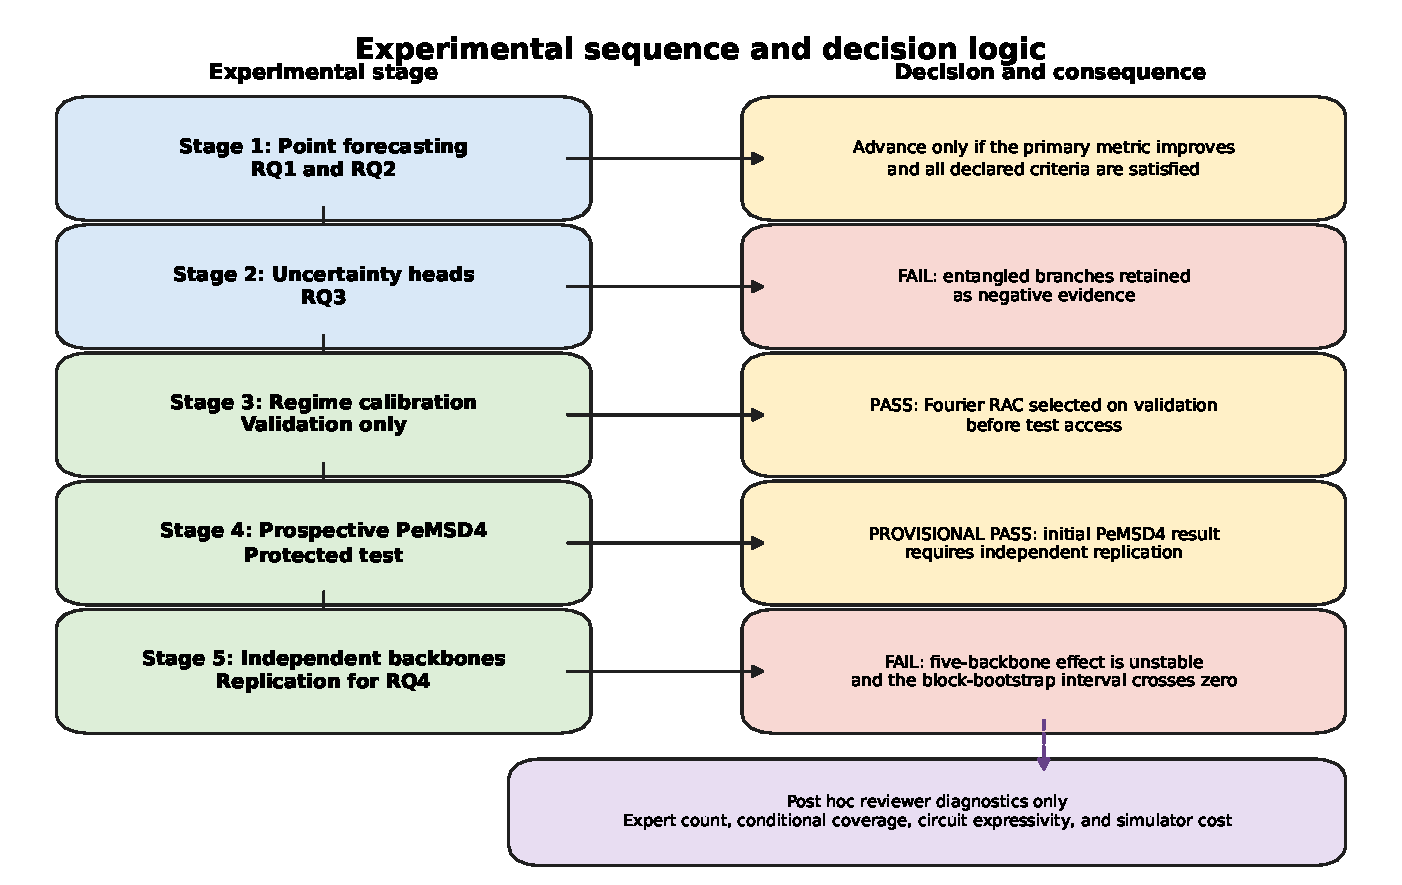
\includegraphics[width=\textwidth]{figures/figure07_experimental_flow.pdf}
\caption{Experimental sequence and decision logic. Blue boxes denote confirmatory point and uncertainty comparisons, green boxes denote calibration and transfer stages, red boxes denote failed gates, and purple denotes reviewer requested post hoc diagnostics. A gate advances only when the archived primary metric, coverage requirement, and seed consistency rule are all satisfied. A failed branch remains in the evidence record but cannot select a downstream test result.}
\label{fig:experimentflow}
\end{figure*}

\section{QUARTS system architecture and method}\label{sec:method}

\subsection{System overview}\label{subsec:overview}

Figure~\ref{fig:architecture} presents the complete system. A chronological preprocessing stage constructs masked input windows, scales values with training data only, and supplies the network graph and time covariates. The forecasting backbone produces a base trajectory \(B\) and a latent node representation \(H\). A shared calibration head operates on the same representation for every treatment. Depending on the experiment, it estimates an additive point correction, a positive uncertainty scale, or the mixture weights of ordered interval experts. Split conformal or conformal quantile calibration uses only the assigned validation segment. A decision gate then determines whether the branch may progress to a protected test split.

\begin{figure*}[t]
\centering
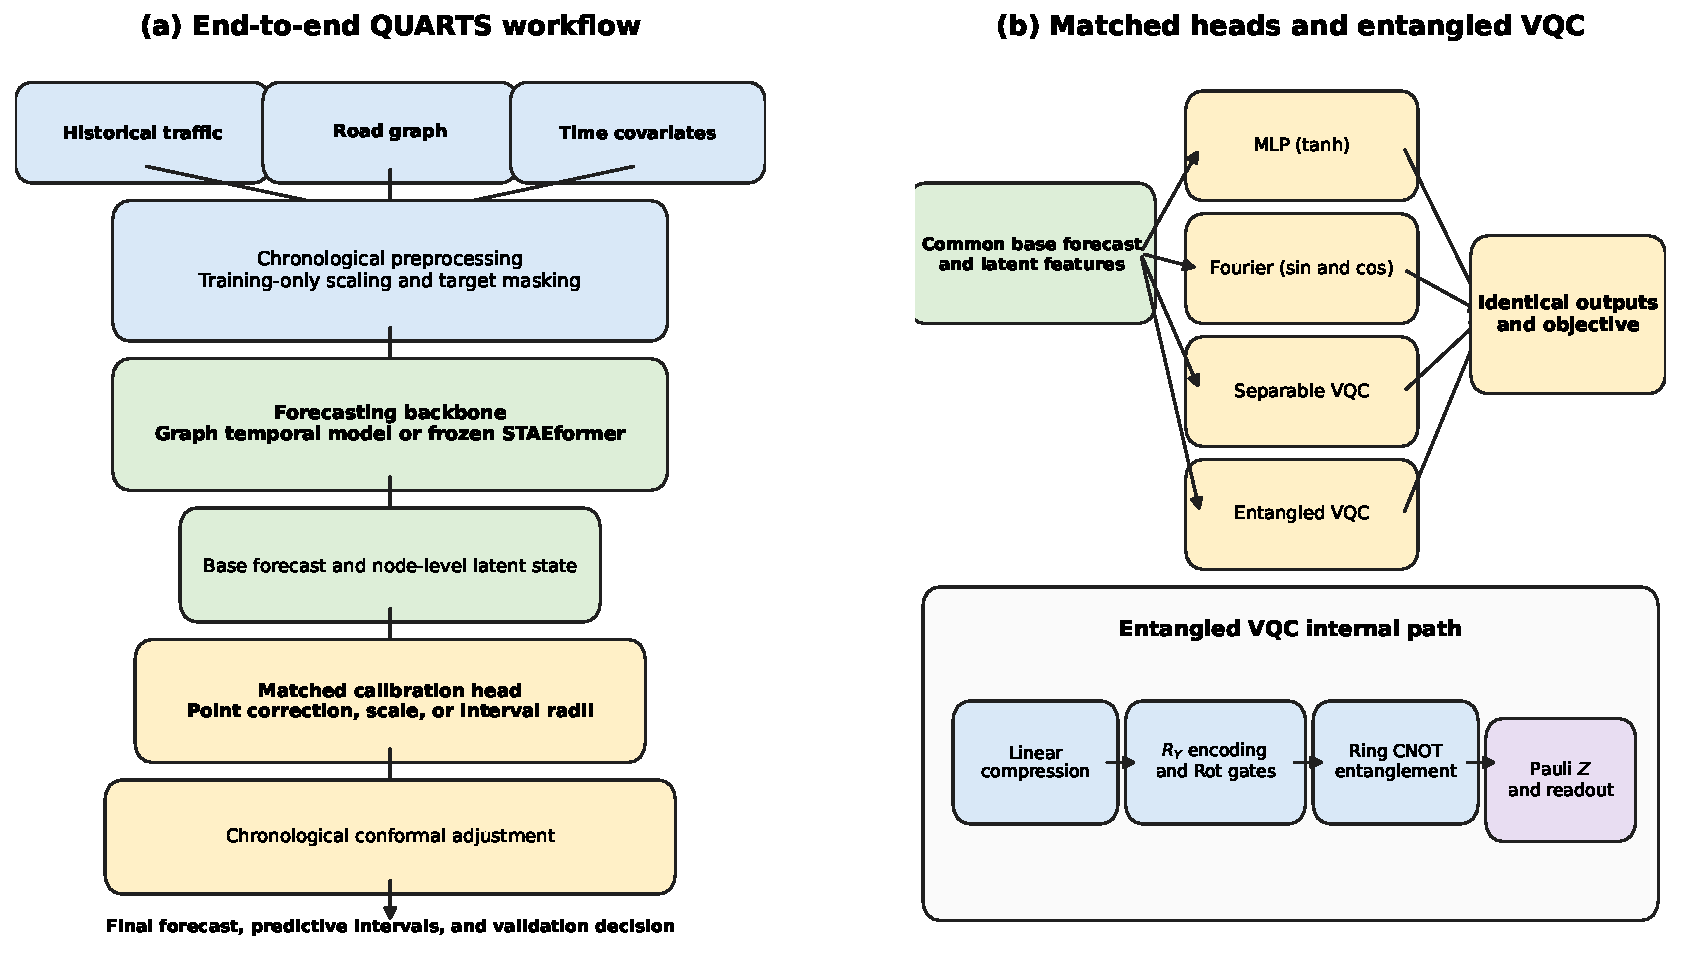
\includegraphics[width=\textwidth]{figures/figure00_system_architecture.pdf}
\caption{QUARTS system architecture. Panel (a) shows the chronological data flow through preprocessing, forecasting, residual calibration, conformal adjustment, and validation. Panel (b) shows the matched calibration head comparison and the internal structure of the entangled variational quantum circuit.}
\label{fig:architecture}
\end{figure*}

\subsection{Forecasting backbones}\label{subsec:backbones}

The reference QUARTS backbone combines graph propagation with a gated recurrent encoder. For an input \(X\), graph propagated features \(AX\) are concatenated with the original features and encoded for every node. A linear horizon head maps the final hidden state \(H\in\mathbb{R}^{N\times d}\) to the base forecast \(B\in\mathbb{R}^{12\times N}\). The unchanged version of this backbone is retained as a control.

The later uncertainty studies use a frozen STAEformer backbone. Freezing is methodologically important because all interval heads then receive identical point forecasts and representations. Any difference in WIS can be attributed to residual calibration rather than to a change in point forecasting capacity. The revised PeMSD4 replication independently trains STAEformer with seeds 17, 42, 73, 101, and 202.

\subsection{Entangled and separable quantum heads}\label{subsec:vqc}

The reference quantum head uses four qubits and depth two. A linear layer compresses each node representation to \(q\) values. The bounded angles are
\begin{equation}
 z=\pi\tanh(W_cH+b_c).
\label{eq:compress}
\end{equation}
At each circuit layer, \(R_Y(z_j)\) reuploads the corresponding feature on qubit \(j\), followed by a trainable \(R_ZR_YR_Z\) rotation. The entangled treatment applies a ring of controlled NOT gates after these local rotations. The separable treatment removes this ring and changes nothing else. Pauli \(Z\) expectation values form the vector \(m\), and a linear readout produces the required horizons:
\begin{equation}
 (\Delta,\widetilde{s})=W_om+b_o,\qquad s=\operatorname{softplus}(\widetilde{s})+\epsilon .
\label{eq:readout}
\end{equation}
For point forecasting, \(\widehat{Y}=B+\Delta\). For scale only experiments, the frozen location remains \(B\). The main experiments use analytic state vector simulation without sampling shots. No claim about execution speed or accuracy on physical quantum hardware is made.

Figure~\ref{fig:circuits} makes the entanglement ablation explicit. Both point heads contain 132 compression parameters, 24 circuit rotation parameters, and 120 readout parameters, giving 276 head parameters and 4,140 parameters when the common backbone is included. The trainable circuit angles are initialized independently from \(\mathcal{U}(0,2\pi)\). Adam, the learning rate $10^{-3}$, weight decay $10^{-4}$, minibatch order, early stopping rule, and five seeds are identical. Each two layer circuit has eight data encoding $R_Y$ operations and eight trainable \(\mathrm{Rot}\) operations, equivalent to 24 elementary trainable rotations. The entangled circuit adds eight fixed CNOT operations. PennyLane resource tracing gives logical depths 12 and 4 for the entangled and separable circuits, respectively. Thus, parameter count is matched, but gate count, depth, computational graph, and expressivity necessarily differ.

As a reviewer requested architecture diagnostic, 256 random input and parameter draws were evaluated without fitting to traffic targets. The entangled circuit had an expressibility divergence from the Haar fidelity distribution of $0.039$, compared with $0.183$ for the separable circuit, and a mean Meyer Wallach entanglement measure of $0.841\pm0.083$, compared with numerical zero for the separable circuit. These values verify that the added ring changes the represented state family. They do not establish useful task specific capacity, and they do not alter the predictive comparison.

\begin{figure*}[t]
\centering
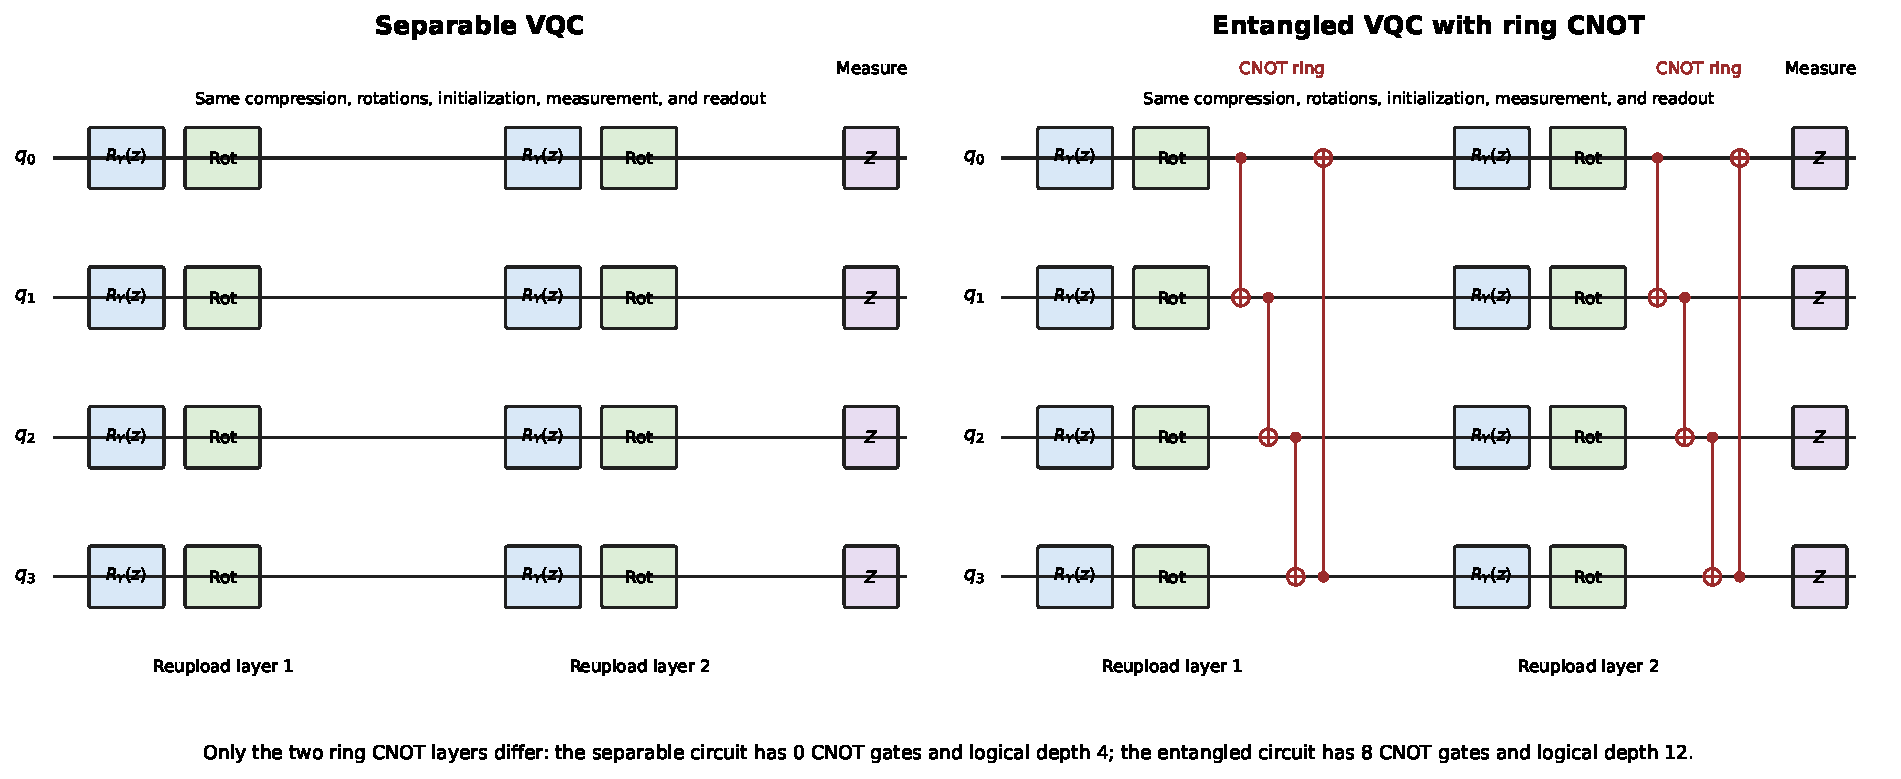
\includegraphics[width=\textwidth]{figures/figure08_circuit_comparison.pdf}
\caption{Side by side circuit structures for the entanglement ablation. Both variational quantum circuits (VQCs) use four qubits, two data reuploading layers, identical $R_Y$ encoding, identical trainable \(\mathrm{Rot}=R_ZR_YR_Z\) gates, Pauli $Z$ measurement, classical readout, initialization, and optimization. The entangled VQC alone contains the eight ring CNOT operations shown in red.}
\label{fig:circuits}
\end{figure*}

\subsection{Classical matched heads}\label{subsec:controls}

The Fourier control receives the same compressed node representation. At layer \(k\), it forms
\begin{equation}
 p_k=\left[\sin(kz+\phi_k),\cos(kz+\phi_k)\right],
 \qquad z\leftarrow\tanh(W_kp_k+b_k).
\label{eq:fourier}
\end{equation}
It therefore exposes periodic functions related to the spectral structure of data reuploading while remaining fully classical. Width was selected to keep its trainable parameter count close to that of the quantum head. The multilayer perceptron uses a compact hyperbolic tangent hidden layer. The unchanged backbone supplies a no calibration control. Together, these treatments distinguish an entanglement effect from periodic nonlinearity, generic nonlinear capacity, and the effect of adding any calibration layer.

\subsection{Regime aware interval calibration}\label{subsec:rac}

The regime aware calibrator contains \(K=3\) shared interval experts. Three experts were fixed before the regime study as a compact low, intermediate, and high residual scale design; the value was not selected by reading test performance. A head maps the node representation to logits, which become mixture weights
\begin{equation}
 \pi_{n,k}=\frac{\exp(g_k(H_n))}
 {\sum_{j=1}^{K}\exp(g_j(H_n))}.
\label{eq:gate}
\end{equation}
Positive increments are summed in reverse order to obtain nested radii for the three interval levels. The mixture of expert radii produces \(r^{(\alpha)}\), and the symmetric interval is \(B\pm r^{(\alpha)}\). The asymmetric extension learns separate lower and upper increments. The ordered construction prevents a nominally wider interval from being contained inside a narrower one.

After training, horizon and level specific conformal factors are estimated from a dedicated chronological calibration segment. For horizon $h$, level \(\alpha\), residual $e_i=|Y_i-B_i|$, and uncalibrated radius $r_i^{(\alpha)}$, the nonconformity score is $e_i/r_i^{(\alpha)}$. Its finite sample upper quantile multiplies future radii. Calibration is separate by horizon and interval level, but pooled over nodes within the assigned chronological segment. Symmetric adaptive conformal quantile residual calibration (SA-CQR) instead trains lower and upper residual quantiles with pinball loss and applies an additive conformity correction. These procedures calibrate the frozen forecast rather than altering its location.

The chronological construction prevents future observations from entering model fitting or calibration, but it does not make overlapping traffic windows exchangeable. Reported coverage is therefore empirical marginal coverage on the indicated future segment, not a distribution free conditional guarantee. Temporal dependence is addressed in uncertainty estimates by resampling complete daily blocks, while distribution drift remains a threat that requires rolling or adaptive recalibration in deployment.

\subsection{Objectives and evaluation measures}\label{subsec:metrics}

Point performance is reported with mean absolute error, root mean squared error, and weighted absolute percentage error. For observed targets \(\mathcal{I}=\{i:M_i=1\}\),
\begin{equation}
 \operatorname{MAE}=\frac{1}{|\mathcal{I}|}\sum_{i\in\mathcal{I}}
 |Y_i-\widehat{Y}_i|.
\label{eq:mae}
\end{equation}
For a central interval \([L_\alpha,U_\alpha]\), the interval score is
\begin{equation}
 \operatorname{IS}_{\alpha}=(U_\alpha-L_\alpha)
 +\frac{2}{\alpha}(L_\alpha-Y)\mathbf{1}\{Y<L_\alpha\}
 +\frac{2}{\alpha}(Y-U_\alpha)\mathbf{1}\{Y>U_\alpha\}.
\label{eq:is}
\end{equation}
The WIS used in training and evaluation combines absolute error at the location with interval scores at \(\alpha\in\{0.1,0.2,0.5\}\), using the conventional \(\alpha/2\) weights \cite{bracher2021wis}. Lower WIS is better. The \(90\%\) empirical coverage and mean width are reported beside WIS so that score changes can be interpreted.

\section{Experimental design}\label{sec:experiment}

\subsection{Datasets and preprocessing}\label{subsec:data}

Table~\ref{tab:datasets} summarizes the four public traffic networks. METR-LA and PEMS-BAY contain speed measurements from 207 and 325 sensors. PeMSD4 and PeMSD8 contain traffic measurements from 307 and 170 detectors. All series use five minute sampling. METR-LA includes 34,272 time steps from March to June 2012, PEMS-BAY includes 52,116 time steps from January to June 2017, and PeMSD4 includes 16,992 time steps from January to February 2018. The dataset audit found no not a number values in METR-LA, although \(8.109\%\) of entries were zero and were masked according to the established preprocessing convention.

\begin{table}[t]
\caption{Traffic datasets and their role in the study.}\label{tab:datasets}
\centering
\small
\begin{tabular}{lrrrrl}
\toprule
Dataset & Sensors & Steps & Input & Horizon & Role \\
\midrule
METR-LA & 207 & 34,272 & 12 & 12 & Confirmatory and development \\
PEMS-BAY & 325 & 52,116 & 12 & 12 & Confirmatory \\
PeMSD4 & 307 & 16,992 & 12 & 12 & Prospective replication \\
PeMSD8 & 170 & 17,856 & 12 & 12 & Validation transfer \\
\bottomrule
\end{tabular}
\end{table}

Every dataset was divided chronologically into \(70\%\) training, \(10\%\) validation, and \(20\%\) test partitions. Scaling statistics were calculated from the training partition only. Sliding windows did not cross partition boundaries. The validation partition was subdivided when early stopping, conformal calibration, and held out validation were all required. Test observations were never used to fit head parameters or conformal factors.

\begin{table*}[t]
\caption{Target domain data use. Percentages within validation refer to consecutive, nonoverlapping chronological windows. The PeMSD4 subgroup results added during revision are descriptive analyses of frozen predictions and do not select or recalibrate a model.}\label{tab:datause}
\centering
\scriptsize
\resizebox{\textwidth}{!}{%
\begin{tabular}{lllll}
\toprule
Stage & Model fitting & Selection & Calibration & Final evaluation \\
\midrule
METR-LA and PEMS-BAY point study & Training split & Validation split & Not applicable & Protected test split \\
METR-LA RAC & Training split & First 40\% validation & Next 30\% validation & Final 30\% validation \\
PeMSD4 prospective RAC & Training split & First 40\% validation & Next 30\% validation & Protected test split \\
PeMSD4 recent repair & No refitting & None & Last 10\%, 20\%, or 30\% validation & Frozen test predictions \\
PeMSD8 SA-CQR & Training split & First 40\% validation & Rolling validation folds & Later validation folds only \\
\bottomrule
\end{tabular}%
}
\end{table*}

\subsection{Comparators and implementation}\label{subsec:implementation}

The point study includes historical average and persistence references, the unchanged graph temporal backbone, MLP, Fourier, separable quantum, and entangled quantum residual heads, and the official STAEformer implementation. All QUARTS heads use the same hidden representation and twelve horizon outputs. The reference circuit has four qubits and two reuploading layers. The architecture study evaluates \(q\in\{2,4,6\}\) and depths \(d\in\{1,2,3\}\).

Models were trained for at most 30 epochs with Adam, learning rate \(10^{-3}\), weight decay \(10^{-4}\), batch size 256, early stopping patience seven, and minimum improvement \(5\times10^{-4}\). Confirmatory point results use seeds \(17,42,73,101,\) and \(202\). The uncertainty branches use their declared head seeds. The revised independent PeMSD4 study trains complete backbones with the same five seeds.

The comparison spans simple temporal references, a graph recurrent model, a compact multilayer perceptron (MLP), a Fourier network, and a Transformer with adaptive spatial and temporal embeddings. It therefore tests the proposed head against several distinct inductive biases, but it does not constitute a benchmark of every machine learning family. Random forests, XGBoost, and LightGBM do not directly represent the network and horizon structure without an additional feature engineering protocol, so introducing them after test access would create a new and potentially unequal selection exercise. The broader literature shows that tree ensembles and hybrid models can be strong when their representation is appropriate, including recent applications to fatigue and structural response prediction \cite{naeim2025fatigue,akbarzadeh2025fragility,akbarzadeh2026multihazard}. The conclusion here is consequently restricted to the tested residual interface and backbones rather than generalized to all classical learning approaches.

\begin{table*}[t]
\caption{Optimization and tuning disclosure. The official STAEformer architecture was adopted without an architecture search. The nine quantum size configurations form a sensitivity analysis and did not retrospectively replace the four qubit, depth two reference treatment.}\label{tab:tuning}
\centering
\scriptsize
\resizebox{\textwidth}{!}{%
\begin{tabular}{lllllll}
\toprule
Component & Configurations & Optimizer & Learning rate & Weight decay & Maximum epochs & Selection criterion \\
\midrule
QUARTS point heads & None, MLP, Fourier, separable VQC, entangled VQC & Adam & $10^{-3}$ & $10^{-4}$ & 30 & Validation Laplace loss \\
Quantum sensitivity & $q\in\{2,4,6\}$, $d\in\{1,2,3\}$ & Adam & $10^{-3}$ & $10^{-4}$ & 30 & Reported as full grid \\
STAEformer & Official published architecture, one configuration per dataset & Adam & $10^{-3}$ & $3\times10^{-4}$ or $10^{-4}$ & 30 & Validation MAE \\
RAC heads & Constant, MLP, Fourier, separable VQC, entangled VQC & Adam & $3\times10^{-3}$ & 0 & 15 & Chronological validation WIS \\
PeMSD4 backbone and heads & Five backbone seeds, three interval heads & Adam & $10^{-3}$, $3\times10^{-3}$ & $3\times10^{-4}$, 0 & 12, 15 & Validation MAE and WIS \\
\bottomrule
\end{tabular}%
}
\end{table*}

The experiments ran on Windows 11 with Python 3.12.13, PyTorch 2.13.0 built for CUDA 13.0, PennyLane 0.39, NumPy 2.0.2, pandas 2.2.3, SciPy 1.18.0, and scikit learn 1.9.0. The GPU was an NVIDIA GeForce RTX 5060 Laptop GPU with 8,151 MiB of memory. Quantum models were simulated on the same computer, which provides a controlled software comparison but not a hardware quantum benchmark.

\subsection{Statistical analysis}\label{subsec:statistics}

Overall differences among point models were assessed separately for each dataset with the Friedman rank test \cite{friedman1937ranks}. Cliff's delta was recorded as a distribution free descriptive effect size \cite{cliff1993dominance}. The original instance level bootstrap and Wilcoxon calculations are retained in the repository for provenance, but they are no longer used for inferential claims because overlapping windows, nodes, and horizons are strongly correlated.

The revised analysis first averages the paired loss difference over every node and horizon within a five minute forecast origin. It then uses 5,000 circular moving block bootstrap replicates with blocks of 288 consecutive origins, corresponding to one day \cite{efron1979bootstrap}. The primary interval resamples the five independently trained seeds and then resamples daily blocks within each selected seed. This hierarchical construction treats the training seed as the independent replication unit while preserving short range temporal, spatial, and cross horizon dependence inside each origin. Seed means, seed standard deviations, directional wins, and the hierarchical $95\%$ interval are reported together.

For PeMSD4, the same procedure is applied to the origin averaged Fourier minus MLP WIS. Coverage and width are summarized at seed level rather than inferred from more than one million correlated forecast values. Conditional results by horizon, traffic intensity, detector, base residual, local volatility, and dominant expert are descriptive post hoc diagnostics. The decision does not rest on a small instance level $p$ value; it requires practical magnitude, directional consistency across independent backbones, and the archived coverage range.

\subsection{Experiment gates}\label{subsec:gates}

The study followed a staged sequence. Point forecasting first tested whether the entangled head warranted promotion. The QUARTS uncertainty module (QUARTS-UQ) then isolated uncertainty scale prediction. The QUARTS regime aware calibrator (QUARTS-RAC) tested regime selection on validation data. Residual adaptive quantile calibration (RAQ) tested asymmetric intervals. A favourable Fourier result was next evaluated prospectively on PeMSD4 and was originally repeated with two additional independently trained backbones. Recent conformal repair and SA-CQR transfer were conducted only after the corresponding failure was observed. During revision, PeMSD4 replication was expanded to five backbones, but this post hoc robustness analysis did not change the frozen heads, calibration rules, or protected test predictions. The expert count and conditional calibration analyses are also post hoc diagnostics. Table~\ref{tab:gates} in Section~\ref{sec:results} reports every decision, including failed branches.

\section{Results}\label{sec:results}

\subsection{Confirmatory point forecasting}\label{subsec:pointresults}

Table~\ref{tab:point} and Figure~\ref{fig:point} show the five seed results. Entangled QUARTS obtained MAE \(3.8969\) on METR-LA and \(2.0295\) on PEMS-BAY. The unchanged graph temporal backbone was better on both datasets. STAEformer obtained \(2.9302\) and \(1.5394\), making the entangled head \(32.99\%\) and \(31.84\%\) worse. The result rejects RQ1 for the tested architecture.

\begin{table*}[t]
\caption{Confirmatory point forecasting over five seeds. Values are mean with standard deviation in parentheses. Lower values are better.}\label{tab:point}
\centering
\small
\resizebox{\textwidth}{!}{%
\begin{tabular}{llccc}
\toprule
Dataset & Model & MAE & RMSE & MAPE (\%) \\
\midrule
\multirow{6}{*}{METR-LA}
& Unchanged backbone & 3.8763 (0.0014) & 7.7322 (0.0097) & 10.9696 (0.0437) \\
& MLP head & 3.9003 (0.0079) & 7.8123 (0.0200) & 11.1479 (0.0760) \\
& Fourier head & 3.9039 (0.0035) & 7.8275 (0.0172) & 11.1575 (0.0456) \\
& Separable VQC & 3.8923 (0.0064) & 7.7948 (0.0163) & 11.0770 (0.0483) \\
& Entangled VQC & 3.8969 (0.0054) & 7.8023 (0.0122) & 11.1382 (0.0539) \\
& STAEformer & \textbf{2.9302} (0.0077) & \textbf{5.9603} (0.0144) & \textbf{8.0754} (0.0185) \\
\midrule
\multirow{6}{*}{PEMS-BAY}
& Unchanged backbone & 1.9909 (0.0023) & 4.6805 (0.0161) & 4.5131 (0.0189) \\
& MLP head & 2.0305 (0.0059) & 4.8128 (0.0140) & 4.6246 (0.0269) \\
& Fourier head & 2.0376 (0.0052) & 4.8505 (0.0240) & 4.5999 (0.0216) \\
& Separable VQC & 2.0248 (0.0036) & 4.8021 (0.0067) & 4.5813 (0.0278) \\
& Entangled VQC & 2.0295 (0.0043) & 4.8222 (0.0290) & 4.5735 (0.0194) \\
& STAEformer & \textbf{1.5394} (0.0023) & \textbf{3.5527} (0.0112) & \textbf{3.4520} (0.0293) \\
\bottomrule
\end{tabular}%
}
\end{table*}

\begin{figure}[t]
\centering
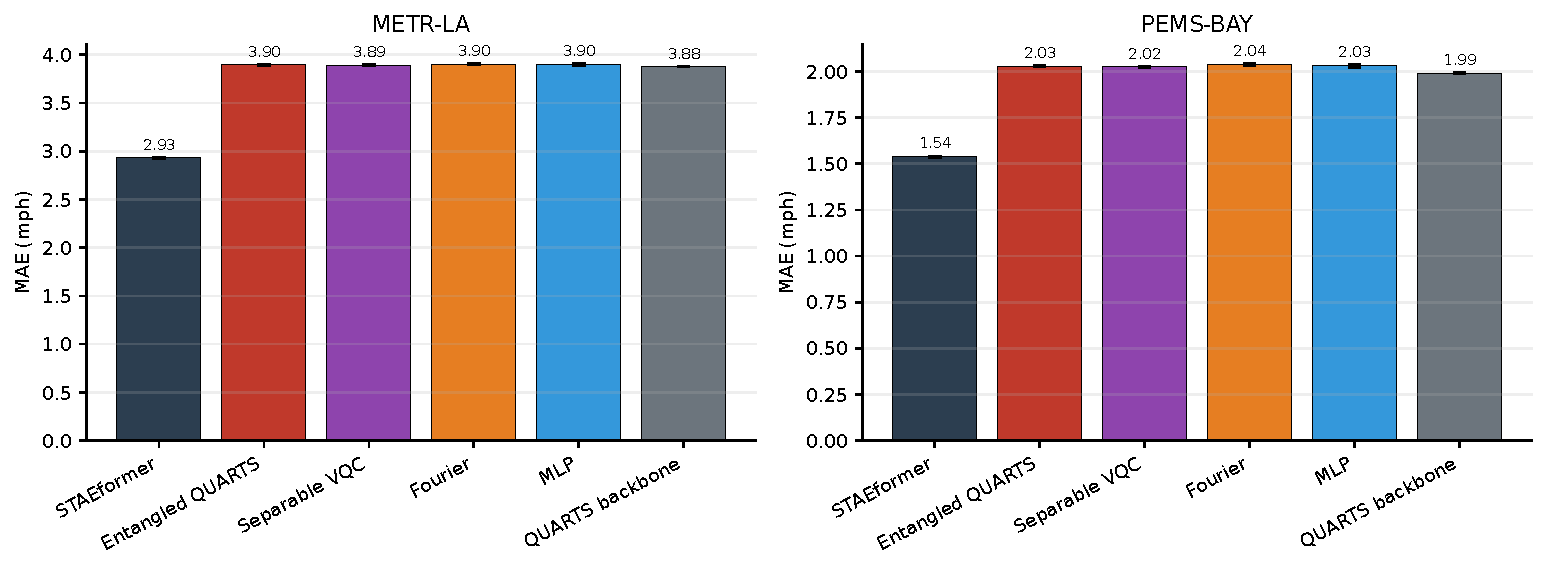
\includegraphics[width=\linewidth]{figures/figure01_confirmatory_point_forecasting.pdf}
\caption{Confirmatory MAE and RMSE on METR-LA and PEMS-BAY. Error bars summarize variation across five seeds.}
\label{fig:point}
\end{figure}

The matched comparisons answer RQ2. Entangled QUARTS was \(0.120\%\) worse than the separable circuit on METR-LA and \(0.233\%\) worse on PEMS-BAY. It was \(0.178\%\) and \(0.397\%\) better than Fourier. These differences are small relative to the gap from STAEformer and do not establish an entanglement benefit. Under the revised hierarchical daily block bootstrap, the entangled minus separable MAE difference was $0.0048\pm0.0073$ across seeds on METR-LA, with $95\%$ interval \([-0.0017,0.0104]\), and $0.0047\pm0.0066$ on PEMS-BAY, with interval \([0.0002,0.0106]\). The quantum head won one of five and two of five seed comparisons, respectively. The entangled minus Fourier differences were \(-0.0068\pm0.0074\), with interval \([-0.0129,-0.0011]\), and \(-0.0081\pm0.0079\), with interval \([-0.0140,-0.0017]\). Although both Fourier intervals exclude zero, the changes are below $0.01$ MAE, reverse for one seed on each dataset, and occur while the unchanged backbone remains better. The Friedman tests rejected equality among all treatments on METR-LA (\(\chi^2_F=21.23\), \(p=0.00073\)) and PEMS-BAY (\(\chi^2_F=20.43\), \(p=0.00104\)), a result driven primarily by the much larger difference from STAEformer.

\begin{figure}[t]
\centering
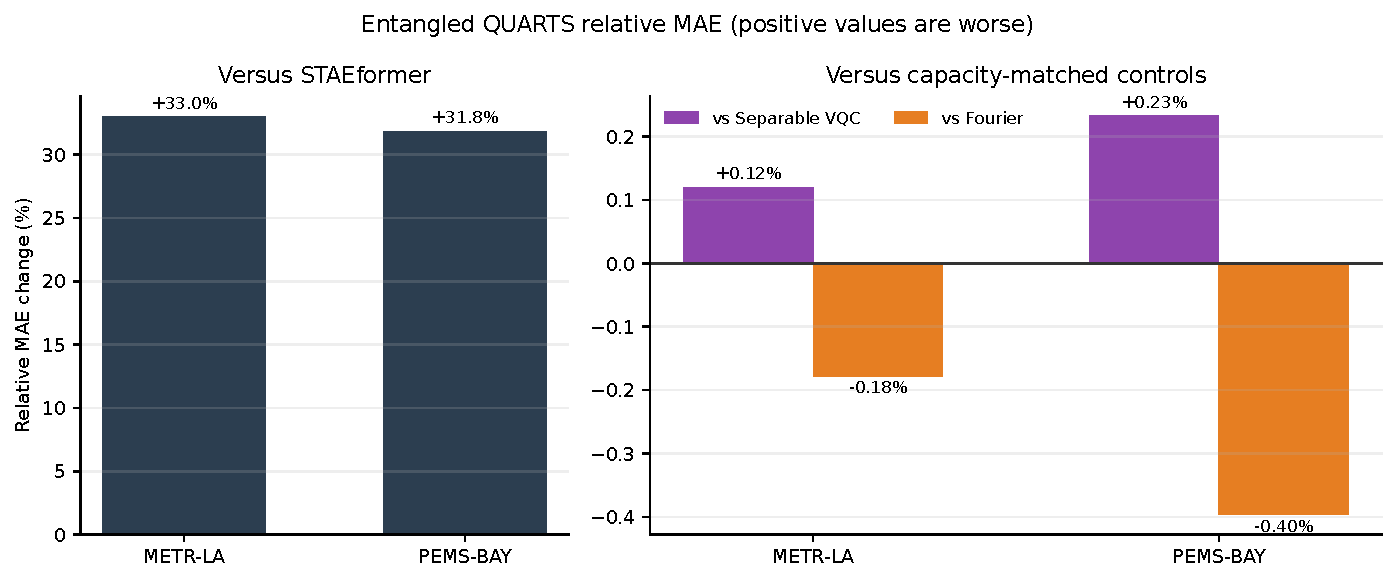
\includegraphics[width=\linewidth]{figures/figure02_quantum_matched_control_effects.pdf}
\caption{Relative effects of the entangled quantum head against matched controls. Values near zero indicate that the compared heads behave similarly.}
\label{fig:effects}
\end{figure}

\begin{table*}[t]
\caption{Dependence aware paired point comparison. Differences are entangled VQC minus comparator MAE, so negative values favour the entangled head. The interval uses 5,000 hierarchical bootstrap replicates over five training seeds and 288 origin daily blocks.}\label{tab:blockpoint}
\centering
\small
\begin{tabular}{llrrr}
\toprule
Dataset & Comparator & Mean difference & Seed SD & Hierarchical 95\% interval \\
\midrule
METR-LA & Separable VQC & 0.0048 & 0.0073 & \([-0.0017,0.0104]\) \\
METR-LA & Fourier & \(-0.0068\) & 0.0074 & \([-0.0129,-0.0011]\) \\
METR-LA & STAEformer & 0.9857 & 0.0124 & \([0.9292,1.0426]\) \\
PEMS-BAY & Separable VQC & 0.0047 & 0.0066 & \([0.0002,0.0106]\) \\
PEMS-BAY & Fourier & \(-0.0081\) & 0.0079 & \([-0.0140,-0.0017]\) \\
PEMS-BAY & STAEformer & 0.4906 & 0.0050 & \([0.4510,0.5294]\) \\
\bottomrule
\end{tabular}
\end{table*}

\subsection{Architecture and efficiency}\label{subsec:efficiency}

Increasing circuit size did not produce a monotonic accuracy gain. Across nine METR-LA configurations, MAE ranged from \(3.8839\) to \(3.9046\). The best value occurred with six qubits and one layer, while six qubits and deeper circuits were slightly worse. Inference time increased from \(1.069\) s for two qubits and one layer to \(16.760\) s for six qubits and three layers. The corresponding state vector dimension rises from $2^2=4$ to $2^6=64$, and the ring contributes $qd$ CNOT operations per circuit. The reference four qubit, depth two quantum head contained 4,140 trainable parameters, close to the Fourier head's 4,196 parameters. Nevertheless, its METR-LA total training time was \(1,544.3\) s compared with \(162.2\) s for Fourier.

The simulator executed 3,267 batched quantum forward calls, representing 171,388,134 node level state vector circuit instances, for one 30 epoch METR-LA seed. The corresponding PEMS-BAY counts were 4,961 batched calls and 409,428,825 circuit instances. Peak allocated GPU memory was 2.22 GiB and 3.44 GiB, and test inference took 4.54 s and 12.50 s, respectively. These counts describe analytic differentiation and batched state vector evaluation on a classical GPU. They are neither physical quantum processor execution counts nor evidence of hardware speed, memory, or energy efficiency. Figure~\ref{fig:efficiency} places measured simulator costs beside accuracy.

\begin{figure}[t]
\centering
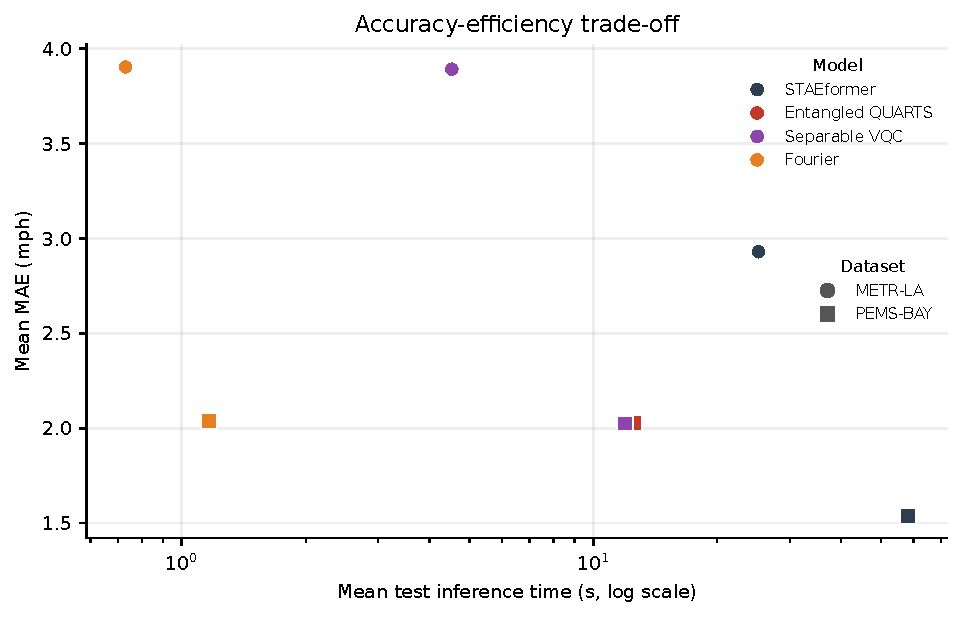
\includegraphics[width=\linewidth]{figures/figure06_accuracy_efficiency_tradeoff.pdf}
\caption{Accuracy and measured computational cost for the confirmatory models. Times refer to the local NVIDIA GPU and analytic state vector simulator. They do not estimate runtime on quantum hardware. Error bars summarize the five training seeds where available.}
\label{fig:efficiency}
\end{figure}

\begin{table*}[t]
\caption{Controlled model size and measured cost. Training and test inference times are mean and standard deviation over five seeds on the same GPU. STAEformer was trained end to end; the residual heads include their common graph temporal backbone. These computational budgets are not equivalent in capacity, so accuracy is interpreted together with the matched head comparisons.}\label{tab:resources}
\centering
\scriptsize
\resizebox{\textwidth}{!}{%
\begin{tabular}{llrrrr}
\toprule
Dataset & Model & Parameters & Training time (s) & Inference time (s) & MAE \\
\midrule
METR-LA & Fourier & 4,196 & $162.2\pm44.9$ & $0.73\pm0.25$ & 3.9039 \\
METR-LA & Separable VQC & 4,140 & $1,539.9\pm6.0$ & $4.53\pm0.02$ & 3.8923 \\
METR-LA & Entangled VQC & 4,140 & $1,544.3\pm1.0$ & $4.54\pm0.02$ & 3.8969 \\
METR-LA & STAEformer & 1,258,980 & $6,850.9\pm201.5$ & $25.19\pm0.30$ & 2.9302 \\
PEMS-BAY & Fourier & 4,196 & $291.9\pm0.2$ & $1.16\pm0.02$ & 2.0376 \\
PEMS-BAY & Separable VQC & 4,140 & $3,792.6\pm145.7$ & $11.96\pm1.06$ & 2.0248 \\
PEMS-BAY & Entangled VQC & 4,140 & $3,947.7\pm6.9$ & $12.57\pm0.07$ & 2.0295 \\
PEMS-BAY & STAEformer & 1,372,260 & $15,694.6\pm2,239.5$ & $58.14\pm3.57$ & 1.5394 \\
\bottomrule
\end{tabular}
}
\end{table*}

\subsection{Uncertainty and regime calibration}\label{subsec:uqresults}

Figure~\ref{fig:uq} consolidates the uncertainty stages. On METR-LA, QUARTS-UQ produced WIS \(2.0045\) and \(89.89\%\) coverage. The separable circuit achieved a slightly lower WIS of \(1.9999\), so the entangled proposal was \(0.23\%\) worse and failed its required \(5\%\) improvement gate. In the validation only regime study, Fourier-RAC obtained the best WIS, \(1.6869\), with \(90.65\%\) coverage. Entangled RAC obtained \(1.6986\), \(0.70\%\) worse than Fourier. The asymmetric Fourier variant increased WIS from \(1.6869\) to \(1.7267\) and raised coverage to \(92.17\%\). It therefore failed both the score and coverage criteria.

\begin{figure*}[t]
\centering
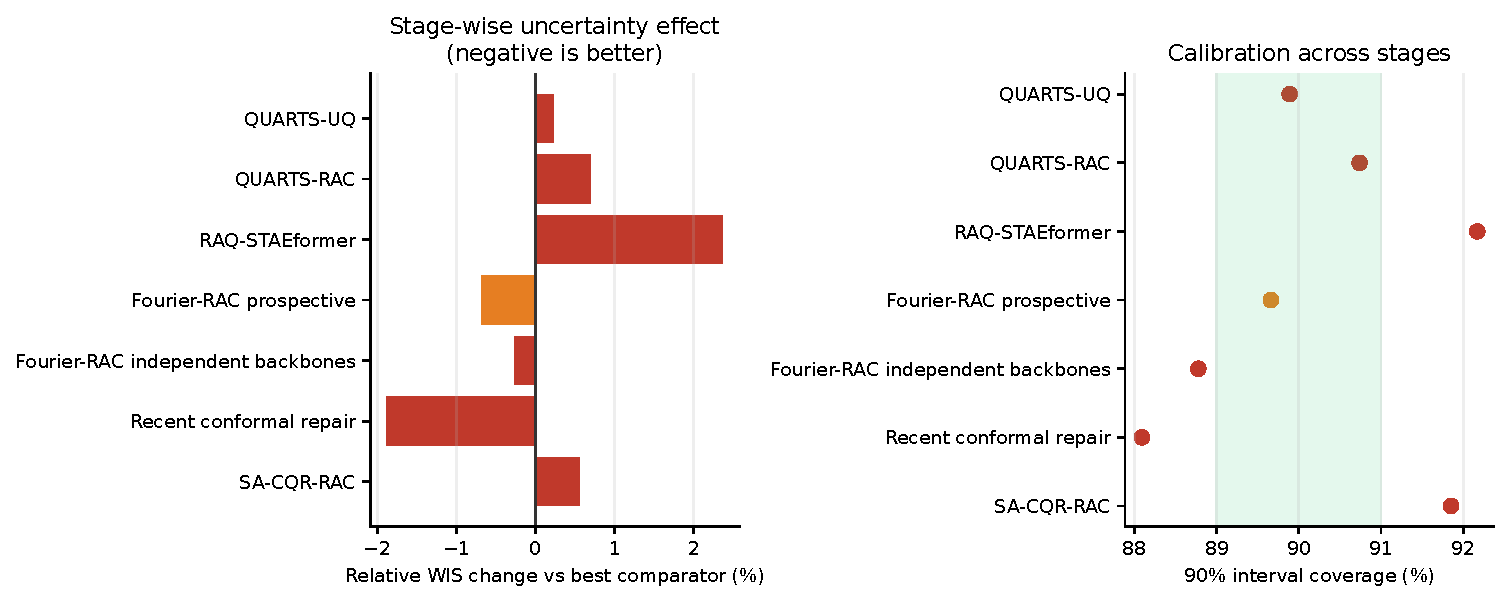
\includegraphics[width=\textwidth]{figures/figure03_uncertainty_stage_synthesis.pdf}
\caption{Synthesis of the uncertainty experiments. WIS is evaluated together with \(90\%\) empirical coverage and the decision status of each stage.}
\label{fig:uq}
\end{figure*}

These findings answer RQ3 for METR-LA. Conditional calibration improved over a constant interval model, but the improvement was classical rather than quantum. Symmetric radii were more reliable than the tested asymmetric extension. A gated point correction initialized near the unchanged STAEformer prediction also produced MAE values between \(2.9276\) and \(2.9277\) for all learned heads, so it did not create a meaningful point forecasting gain.

The reviewer requested expert count ablation used only the chronologically partitioned METR-LA validation data. Mean WIS for $K=1,2,3,4,$ and $5$ was $1.8920$, $1.6899$, $1.6869$, $1.6856$, and $1.6869$, respectively. The corresponding $90\%$ coverage values ranged from $0.9048$ to $0.9101$. Thus one expert was inadequate, while the difference among two to five experts was at most $0.0042$ WIS. The prespecified $K=3$ model used an effective $2.07\pm0.18$ experts and had mean weights $[0.745,0.096,0.158]$ across three head seeds. The routing was concentrated but not collapsed to one expert. Increasing $K$ raised parameter count from 223 at $K=1$ to 383 at $K=5$ without a material score improvement.

\subsection{Prospective PeMSD4 evaluation}\label{subsec:pems4}

The Fourier regime calibrator was selected before opening the PeMSD4 test split. With backbone seed 42, its WIS was \(26.8820\), compared with \(31.4672\) for constant intervals and \(27.0663\) for MLP-RAC. These values correspond to improvements of \(14.58\%\) and \(0.68\%\), and Fourier coverage was \(89.66\%\). This was the strongest prospective result, but its small margin over MLP required independent replication.

The original replication used seeds 42, 73, and 202. Mean Fourier WIS was \(22.6892\), compared with \(22.7480\) for MLP, but seed 202 reversed the ordering and mean Fourier coverage was \(88.78\%\). Figure~\ref{fig:pems4} preserves this original evidence. The reviewer requested expansion added complete backbones for seeds 17 and 101. Across all five backbones, Fourier WIS was $21.2373\pm3.4720$, compared with $21.2681\pm3.5345$ for MLP. Fourier minus MLP was $-0.0308\pm0.1285$ across seeds, with a hierarchical daily block bootstrap $95\%$ interval of $[-0.1336,0.0767]$. Fourier won for seeds 17, 42, and 73, while MLP won for seeds 101 and 202. Mean Fourier coverage was $89.44\%\pm1.70\%$ and mean width was $141.47\pm19.55$. The average coverage therefore entered the declared range after expansion, but the uncertain effect and two directional reversals still failed the robustness gate.

\begin{figure*}[t]
\centering
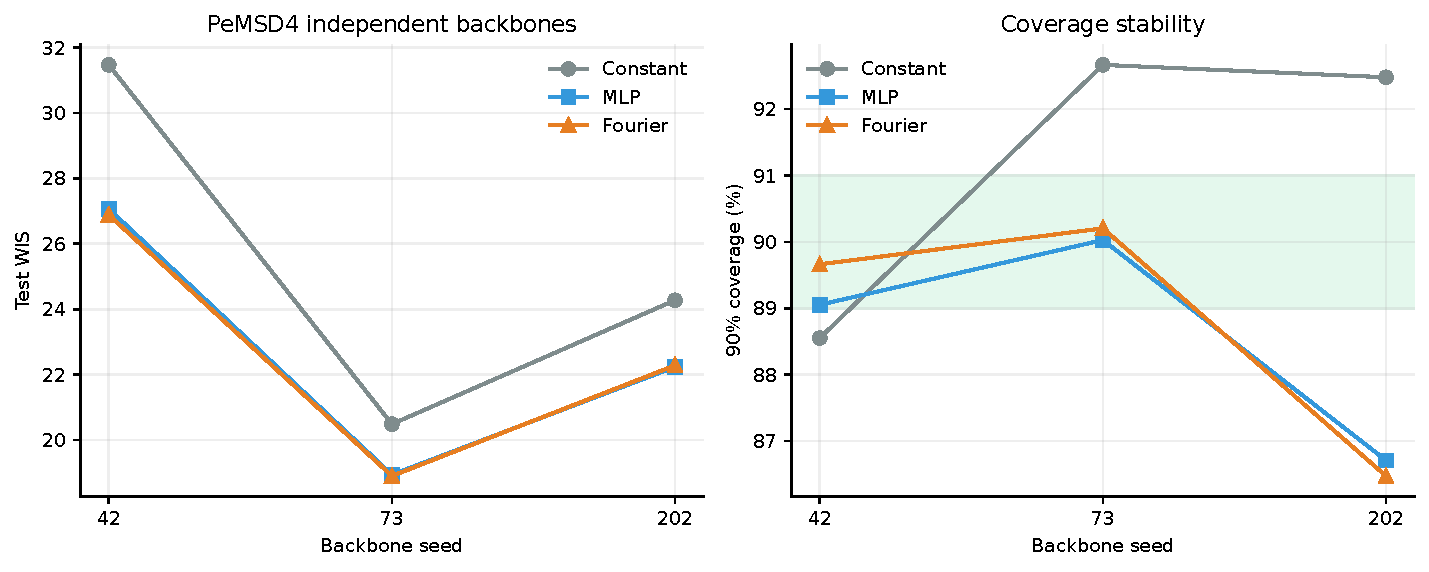
\includegraphics[width=\textwidth]{figures/figure04_pemsd4_independent_backbones.pdf}
\caption{Original PeMSD4 WIS and \(90\%\) coverage for three independently trained STAEformer backbones. The Fourier advantage reverses for seed 202, motivating the reviewer requested expansion to five backbones shown in Figure~\ref{fig:revisiondiagnostics}.}
\label{fig:pems4}
\end{figure*}

Conditional analysis showed why aggregate coverage was insufficient. For Fourier, mean coverage increased from $85.4\%$ at the five minute horizon to $91.8\%$ at 60 minutes. It decreased from $96.2\%$ in the lowest traffic intensity quartile to $83.8\%$ in the highest, while mean width increased from $104.65$ to $197.10$. Coverage in the largest backbone residual quartile was only $61.0\%$. Across detector and seed combinations, median coverage was $89.63\%$, with an interquartile range from $86.63\%$ to $92.64\%$ and a minimum of $72.58\%$. Dominant expert routing was also concentrated: the first Fourier expert was dominant for approximately $98\%$ of PeMSD4 node origins, while the rare second and third experts were associated with higher traffic, local volatility, and backbone residuals. This indicates partial soft mixture use but not three balanced semantic regimes.

\begin{figure*}[t]
\centering
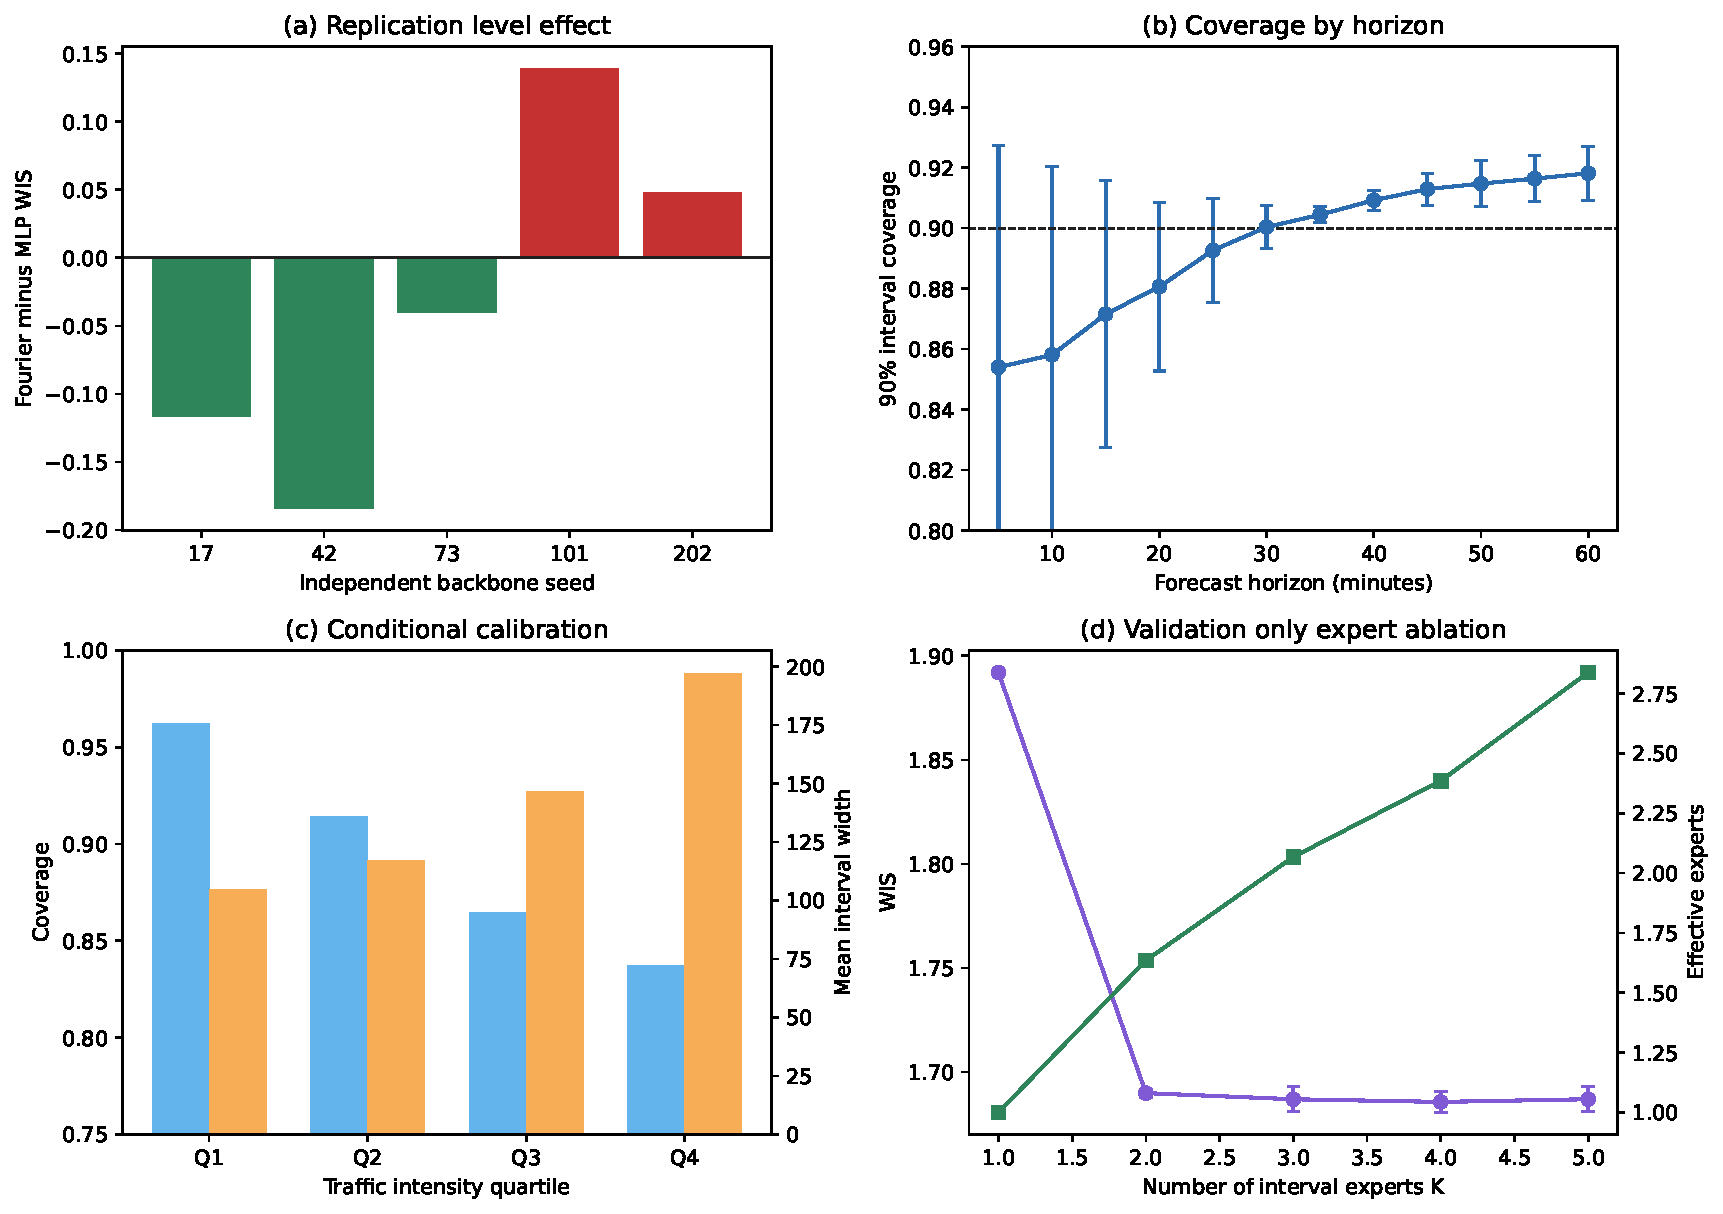
\includegraphics[width=\textwidth]{figures/figure09_revision_diagnostics.pdf}
\caption{Reviewer requested post hoc diagnostics. Panel (a) reports Fourier minus MLP WIS for five independently trained PeMSD4 backbones, where negative values favour Fourier. Panel (b) gives mean Fourier $90\%$ coverage by forecast horizon with standard deviation across backbones. Panel (c) compares coverage and mean interval width across traffic intensity quartiles. Panel (d) reports METR-LA validation WIS and effective expert count for $K=1$ to $5$ over three head seeds. These diagnostics do not redefine the prespecified promotion gates.}
\label{fig:revisiondiagnostics}
\end{figure*}

\begin{table}[t]
\caption{Conditional PeMSD4 Fourier interval diagnostics averaged over five backbones. Q1 and Q4 denote the lowest and highest quartiles within each seed. These post hoc summaries expose heterogeneity that is hidden by aggregate coverage.}\label{tab:conditional}
\centering
\scriptsize
\begin{tabular}{llrrr}
\toprule
Condition & Level & WIS & Coverage & Width \\
\midrule
Horizon & 5 min & 18.86 & 0.854 & 113.42 \\
Horizon & 60 min & 25.10 & 0.918 & 178.96 \\
Traffic intensity & Q1 & 12.17 & 0.962 & 104.65 \\
Traffic intensity & Q4 & 32.87 & 0.837 & 197.10 \\
Base residual & Q1 & 8.85 & 1.000 & 117.83 \\
Base residual & Q4 & 47.38 & 0.615 & 195.90 \\
Local volatility & Q1 & 12.69 & 0.956 & 106.19 \\
Local volatility & Q4 & 33.63 & 0.840 & 201.78 \\
\bottomrule
\end{tabular}
\end{table}

\subsection{Calibration repair and PeMSD8 transfer}\label{subsec:transfer}

A recent window conformal diagnostic was evaluated for the failing seed 202 backbone. Increasing the recent calibration fraction from \(10\%\) to \(30\%\) reduced WIS from \(22.4107\) to \(21.9900\), but coverage reached only \(88.09\%\). The repair therefore did not restore the coverage criterion.

The final transfer branch trained symmetric adaptive conformal quantile residual models on PeMSD8. Across three rolling validation folds, CQR-MLP obtained mean WIS \(15.1716\), while CQR-Fourier obtained \(15.2554\) and mean coverage \(91.85\%\). Fourier was \(0.55\%\) worse and overcovered. According to the gate, the canonical PeMSD8 test split remained untouched. This result rejects RQ4 for the proposed transfer. Figure~\ref{fig:transfer} distinguishes the post hoc repair from the protected validation only transfer.

\begin{figure*}[t]
\centering
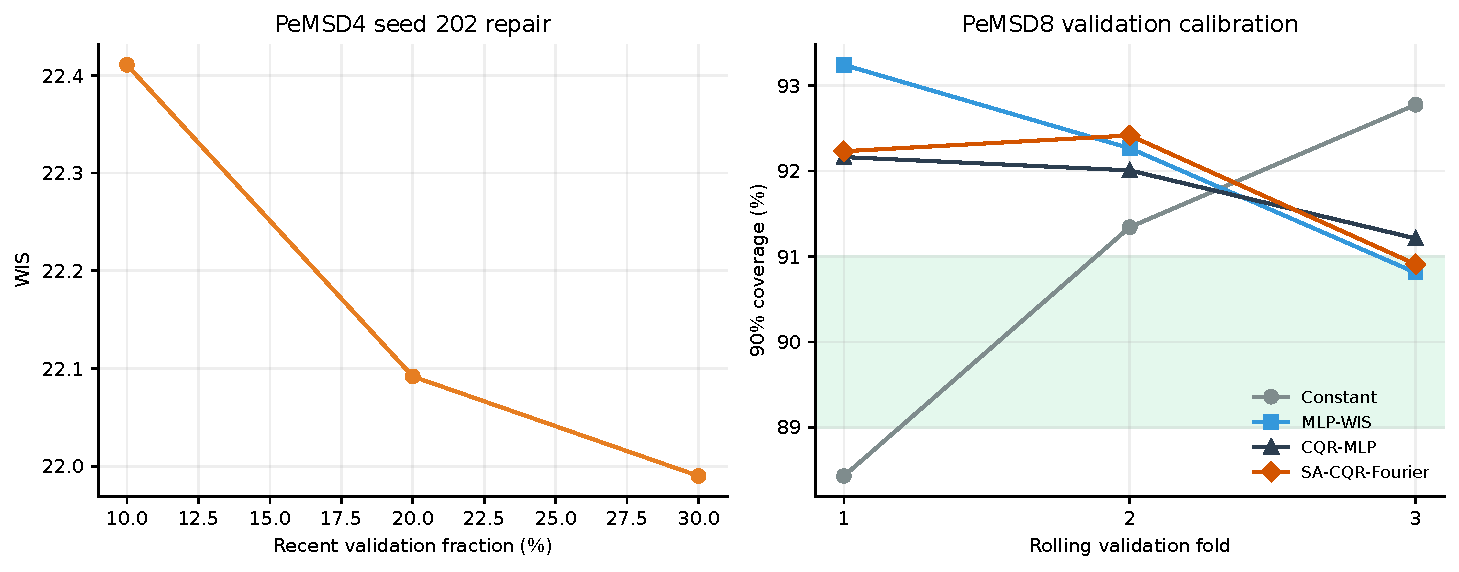
\includegraphics[width=\textwidth]{figures/figure05_calibration_repair_and_transfer.pdf}
\caption{Recent conformal repair on PeMSD4 and validation only SA-CQR transfer to PeMSD8. Neither branch satisfied its complete decision rule.}
\label{fig:transfer}
\end{figure*}

\subsection{Complete gate summary}\label{subsec:gateresults}

Table~\ref{tab:gates} records the selected model, comparator, result, and decision for every stage. No entangled model passed a promotion gate. The prospective Fourier result was encouraging in one run but did not survive the stronger independent backbone criterion. The negative decisions are part of the result rather than discarded tuning attempts.

\begin{table*}[t]
\caption{Experiment gate summary. Relative change is measured against the named comparator, and lower is better for MAE and WIS.}\label{tab:gates}
\centering
\scriptsize
\resizebox{\textwidth}{!}{%
\begin{tabular}{llllrrl}
\toprule
Stage & Data policy & Proposal & Comparator & Proposal & Change (\%) & Decision \\
\midrule
Point forecast & METR-LA test & Entangled VQC & STAEformer & 3.8969 & 32.99 & Fail \\
Point forecast & PEMS-BAY test & Entangled VQC & STAEformer & 2.0295 & 31.84 & Fail \\
QUARTS-UQ & METR-LA exploratory test & Entangled VQC & Separable VQC & 2.0045 & 0.23 & Fail \\
QUARTS-RAC & METR-LA validation & Entangled gate & Fourier gate & 1.6986 & 0.70 & Fail \\
RAQ & METR-LA validation & Asymmetric Fourier & Symmetric Fourier & 1.7267 & 2.36 & Fail \\
Prospective RAC & PeMSD4 test & Fourier gate & MLP gate & 26.8820 & \(-0.68\) & Provisional \\
Independent RAC & PeMSD4, five tests & Fourier gate & MLP gate & 21.2373 & \(-0.14\) & Fail \\
Recent calibration & PeMSD4 diagnostic & Recent Fourier & Ten percent window & 21.9900 & \(-1.88\) & Fail \\
SA-CQR & PeMSD8 validation & CQR-Fourier & CQR-MLP & 15.2554 & 0.55 & Fail \\
\bottomrule
\end{tabular}%
}
\end{table*}

\section{Discussion}\label{sec:discussion}

\subsection{What the controlled comparisons establish}\label{subsec:interpretation}

The principal result is not that a quantum head failed to beat every classical model. It is that changing entanglement changed MAE by less than one quarter of one percent relative to the otherwise identical separable circuit, while both were far behind STAEformer. This pattern does not support an entanglement based explanation. The small improvement over Fourier is likewise insufficient because the unchanged backbone remained better and the effect size was negligible.

The result is consistent with the functional interpretation of data reuploading circuits. Periodic nonlinear features can be useful without being uniquely quantum \cite{schuld2021encoding}. A matched Fourier head exposes this alternative explanation directly. The expressivity diagnostic confirms that the ring CNOT circuit is both more Haar like and able to generate entanglement, while the traffic results show that these state space properties did not translate into a stable predictive gain. The architecture ablation further weakens a capacity argument: additional qubits and layers increased execution time but did not yield a consistent accuracy trend. The experiment cannot prove that entanglement is never useful for traffic data. It establishes only that this \(R_Y\) data reuploading, local \(R_ZR_YR_Z\) ansatz, directed ring topology, and Pauli \(Z\) readout did not provide a stable advantage at two to six qubits and one to three layers.

\subsection{Why the classical interval result did not qualify as final evidence}\label{subsec:replicationdiscussion}

The first PeMSD4 run met its prospective WIS and coverage requirements and improved substantially over constant intervals. That finding demonstrates that the frozen latent state contains information about conditional residual scale. The margin over MLP was only \(0.68\%\), however. Five independent backbones exposed the fragility hidden by a single initialization. Two seeds reversed the ordering, the mean difference shrank to $-0.0308$ WIS, and its hierarchical interval crossed zero. Average coverage entered the accepted range, but conditional analysis revealed substantial undercoverage for high intensity, high volatility, large residual, and selected detector groups.

This distinction matters for large traffic datasets. With more than one million paired forecasts per backbone, a very small mean difference can produce a narrow interval if individual forecasts are treated as independent. Statistical detectability does not guarantee stability across training conditions or practical relevance. The revised decision therefore combines a seed level effect, daily block uncertainty, effect direction, aggregate and conditional coverage, and independent initialization. Under that rule the Fourier model did not qualify as a robust improvement.

\subsection{Implications for quantum transportation research}\label{subsec:implications}

Three design principles follow. First, a quantum component should be assigned a clearly isolated role. A hybrid model that changes its backbone, input features, and optimization at the same time cannot identify the source of an improvement. Second, matched controls should reflect the known function class of the circuit. Parameter matching alone is not enough when a classical periodic layer captures the same spectral bias. Third, protected validation gates should remain active after a favourable result. The untouched PeMSD8 test set is more informative than a selectively reported transfer score because it shows that the stopping rule was respected.

Quantum traffic forecasting may still be valuable when a circuit processes a compact decision state, when data or kernels have a structure suited to a quantum feature map, or when physical hardware changes the computational tradeoff. Alternative amplitude, phase, or problem informed graph encodings, deeper or data dependent ansatzes, nonlocal entangling topologies, and other observables remain outside the tested design space. Those possibilities require hardware aware experiments, noise and shot budgets, strong network backbones, and repeated out of distribution evaluation. The present simulator results do not establish any of them.

\section{Limitations and threats to validity}\label{sec:limitations}

The quantum circuits were executed with analytic state vector simulation on a classical GPU environment. Consequently, runtime, memory, and circuit instance counts describe the implementation used here and cannot predict latency, queueing, compilation overhead, noise, sampling cost, or energy use on quantum hardware. The primary circuits were also small and covered only one encoding, one local ansatz, one ring entangler, and one measurement family. Larger or structurally different circuits could represent different functions, but the observed simulator growth and nonmonotonic ablation make unrestricted scaling an unsupported remedy.

The point experiments use two speed networks, while the later interval studies use PeMSD4 and PeMSD8. This improves dataset diversity but does not cover incidents, weather disruptions, or long term distribution shift. Conformal calibration was applied chronologically and assessed empirically. Dependence between traffic observations means that standard exchangeability based coverage theory does not apply without qualification.

Traffic errors remain dependent across overlapping windows, connected nodes, and horizons. The revised bootstrap aggregates within each forecast origin, resamples daily temporal blocks, and nests those blocks within independently trained seeds. This is more conservative than treating individual forecasts as independent, but five training seeds still provide limited information about the distribution over optimization outcomes. The final PeMSD4 decision therefore emphasizes the seed standard deviation, directional wins, conditional coverage, and practical effect size rather than an instance level significance result.

STAEformer is a strong comparator on the selected datasets, but it is not the only modern forecasting architecture. Results could change with another frozen backbone or a different latent interface. Hyperparameter budgets were intentionally bounded and shared across treatments. A broader search might improve any head, yet it would also increase selection bias unless nested inside a new protected protocol.

Finally, the proposed architecture underwent a sequence of development stages. The record distinguishes confirmatory, exploratory, validation only, prospective, and post hoc analyses, but later hypotheses were informed by earlier outcomes. They should not be interpreted as one untouched confirmatory family. The complete gate table and archived configurations are supplied so readers can reconstruct this chronology.

\section{Reproducibility and open science}\label{sec:reproducibility}

The reproducibility package contains the complete source code, environment records, immutable experiment configurations, dataset integrity audit, seed level outputs, analysis scripts, publication tables, and vector figures. The package is available from the \href{https://github.com/shishirbit/Quantum-Enhanced-Framework-for-Traffic-Speed-Forecasting-with-Calibrated-Uncertainty}{QUARTS repository on GitHub}. The repository commit associated with this manuscript gives commands for recreating every table and figure.

Raw benchmark data are not redistributed when their original terms or standard download routes apply. Instead, the package provides acquisition instructions, expected file layout, dimensions, and cryptographic hashes for the files used in the experiments. Each run stores its dataset, split, seed, model treatment, metrics, timing, and completion state. Smoke tests and the preprotocol batch size 128 run are marked and excluded from publication aggregation.

The main analysis package expects 50 reference runs, 10 official STAEformer runs, and nine circuit ablations. Its completion audit reports no missing run. The reviewer revision package adds five PeMSD4 backbone evaluations, 15 expert count runs, dependence aware bootstrap outputs, conditional calibration tables, circuit diagnostics, and the scripts that regenerate Figures~\ref{fig:experimentflow}, \ref{fig:circuits}, and \ref{fig:revisiondiagnostics}. Validation only results are labelled separately from canonical test results. PeMSD8 test targets are absent by design because the validation gate failed. This absence can be verified from both the experiment ledger and the publication manifest.

\section{Conclusion}\label{sec:conclusion}

QUARTS was designed to test a specific claim under controlled conditions: whether an entangled variational quantum circuit adds useful residual information to network traffic forecasts or predictive intervals. Across METR-LA and PEMS-BAY, it did not improve the unchanged backbone and remained about one third worse than STAEformer. Its differences from separable quantum and Fourier controls were below \(0.40\%\), with negligible effect sizes. Circuit scaling increased cost without a consistent accuracy gain.

For uncertainty prediction, a Fourier regime calibrator achieved the strongest prospective result on one PeMSD4 backbone, reducing WIS by \(14.58\%\) relative to constant intervals and \(0.68\%\) relative to an MLP. Across five independent backbones, the Fourier minus MLP difference was only $-0.0308\pm0.1285$ WIS, its dependence aware interval crossed zero, and MLP was better for two seeds. Aggregate Fourier coverage was $89.44\%$, but it varied materially by horizon, detector, traffic intensity, volatility, and residual size. A recent conformal repair remained undercovered, and a conformal quantile Fourier model failed PeMSD8 validation. The protected test split was therefore not evaluated.

The study finds no empirical basis for attributing a forecasting or calibration advantage to entanglement in the tested system. Its positive result is methodological: strong backbones, functionally matched controls, seed level replication, interval aware metrics, and binding validation gates make a hybrid quantum claim more credible, whether the final evidence is favourable or negative.

\backmatter

\bmhead{Acknowledgements}

The author acknowledges the maintainers of the public benchmark datasets and the open source software used in this study.

\section*{Declarations}

\bmhead{Funding}

The author received no specific funding for this work.

\bmhead{Competing interests}

The author declares that there are no competing interests.

\bmhead{Ethics approval}

Not applicable. The study uses public traffic sensor datasets and does not involve human participants or animals.

\bmhead{Consent to participate}

Not applicable.

\bmhead{Consent for publication}

Not applicable.

\bmhead{Data availability}

The datasets are publicly available from their established benchmark sources. File acquisition instructions and integrity hashes are included in the repository identified in Section~\ref{sec:reproducibility}.

\bmhead{Code availability}

The complete code, configurations, tables, and figures are available from the repository identified in Section~\ref{sec:reproducibility}.

\bmhead{Author contributions}

The author conceived the study, designed the methodology, developed the software, conducted the experiments, curated and analysed the data, validated the results, prepared the figures and tables, wrote the original manuscript, revised the manuscript, and approved the final version for submission.

\begin{appendices}

\section{Supplementary experiment record}\label{app:supplement}

The supplementary figures report horizon specific point errors, missing input robustness, circuit size and simulated noise sensitivity, each uncertainty development stage, prospective replication, and the protected PeMSD8 validation study. Each figure is presented separately so that its caption maps unambiguously to its panels.

\begin{figure*}[t]
\centering
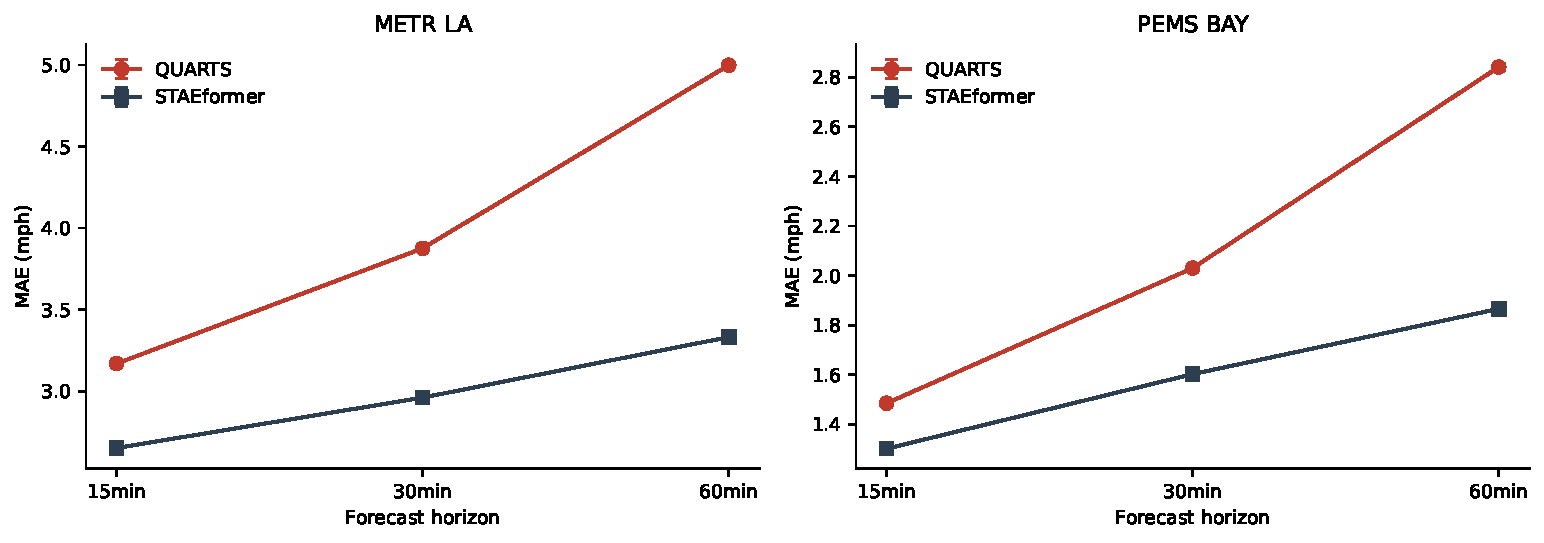
\includegraphics[width=.82\textwidth]{figures/supplement/figureS01_horizon_performance.pdf}
\caption{Horizon specific MAE for confirmatory METR-LA and PEMS-BAY point forecasts. Error bars summarize five training seeds; lower values are better.}
\label{fig:s01}
\end{figure*}

\begin{figure*}[t]
\centering
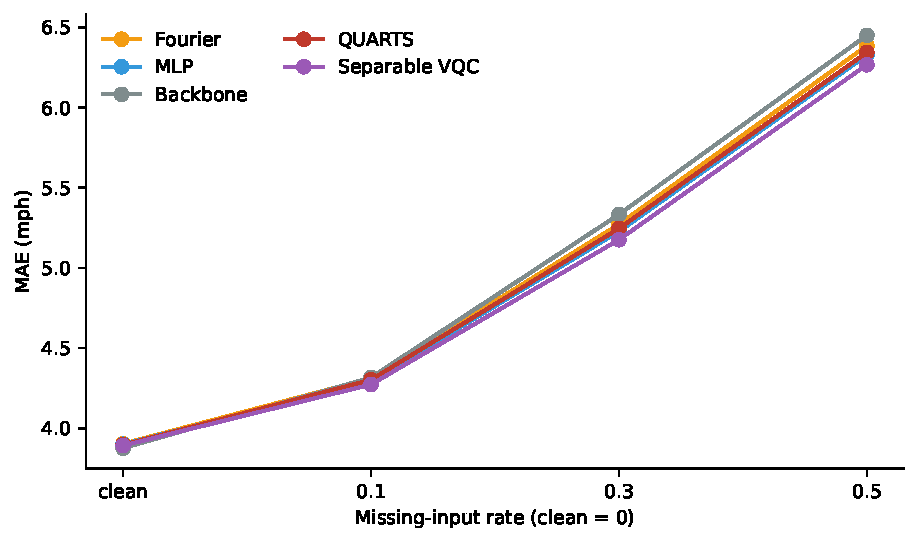
\includegraphics[width=.82\textwidth]{figures/supplement/figureS02_missing_input_metr_la.pdf}
\caption{METR-LA sensitivity to randomly masked input values. The perturbation is applied only to model inputs; target masking and evaluation definitions remain unchanged.}
\label{fig:s02}
\end{figure*}

\begin{figure*}[t]
\centering
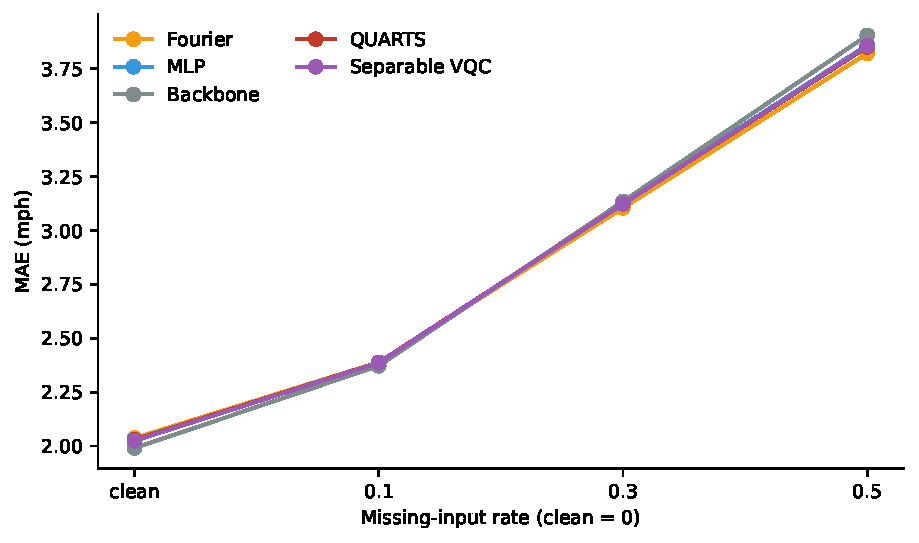
\includegraphics[width=.82\textwidth]{figures/supplement/figureS03_missing_input_pems_bay.pdf}
\caption{PEMS-BAY sensitivity to randomly masked input values under the same perturbation and evaluation protocol as Figure~\ref{fig:s02}.}
\label{fig:s03}
\end{figure*}

\begin{figure*}[t]
\centering
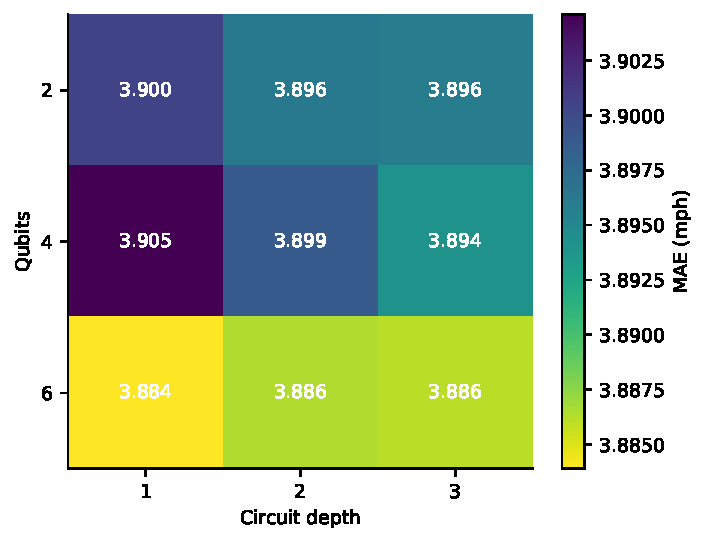
\includegraphics[width=.82\textwidth]{figures/supplement/figureS04_quantum_ablation.pdf}
\caption{Quantum architecture sensitivity on METR-LA across two, four, and six qubits and circuit depths one, two, and three. Accuracy is nonmonotonic while analytic simulator time increases with circuit size.}
\label{fig:s04}
\end{figure*}

\begin{figure*}[t]
\centering
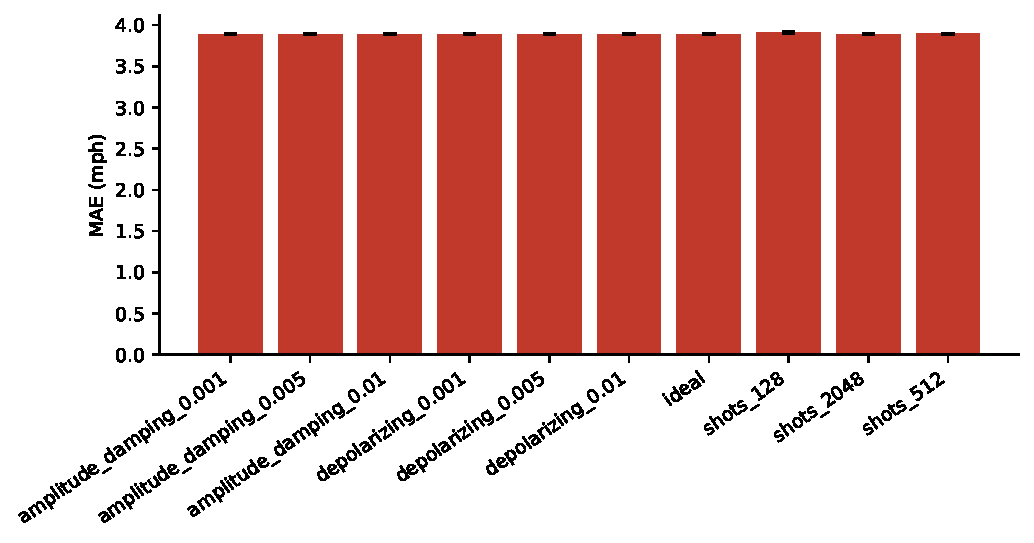
\includegraphics[width=.82\textwidth]{figures/supplement/figureS05_quantum_noise.pdf}
\caption{Sensitivity of the simulated quantum head to the evaluated finite shot, depolarizing, and amplitude damping settings. These are simulator perturbations rather than measurements on physical hardware.}
\label{fig:s05}
\end{figure*}

\begin{figure*}[t]
\centering
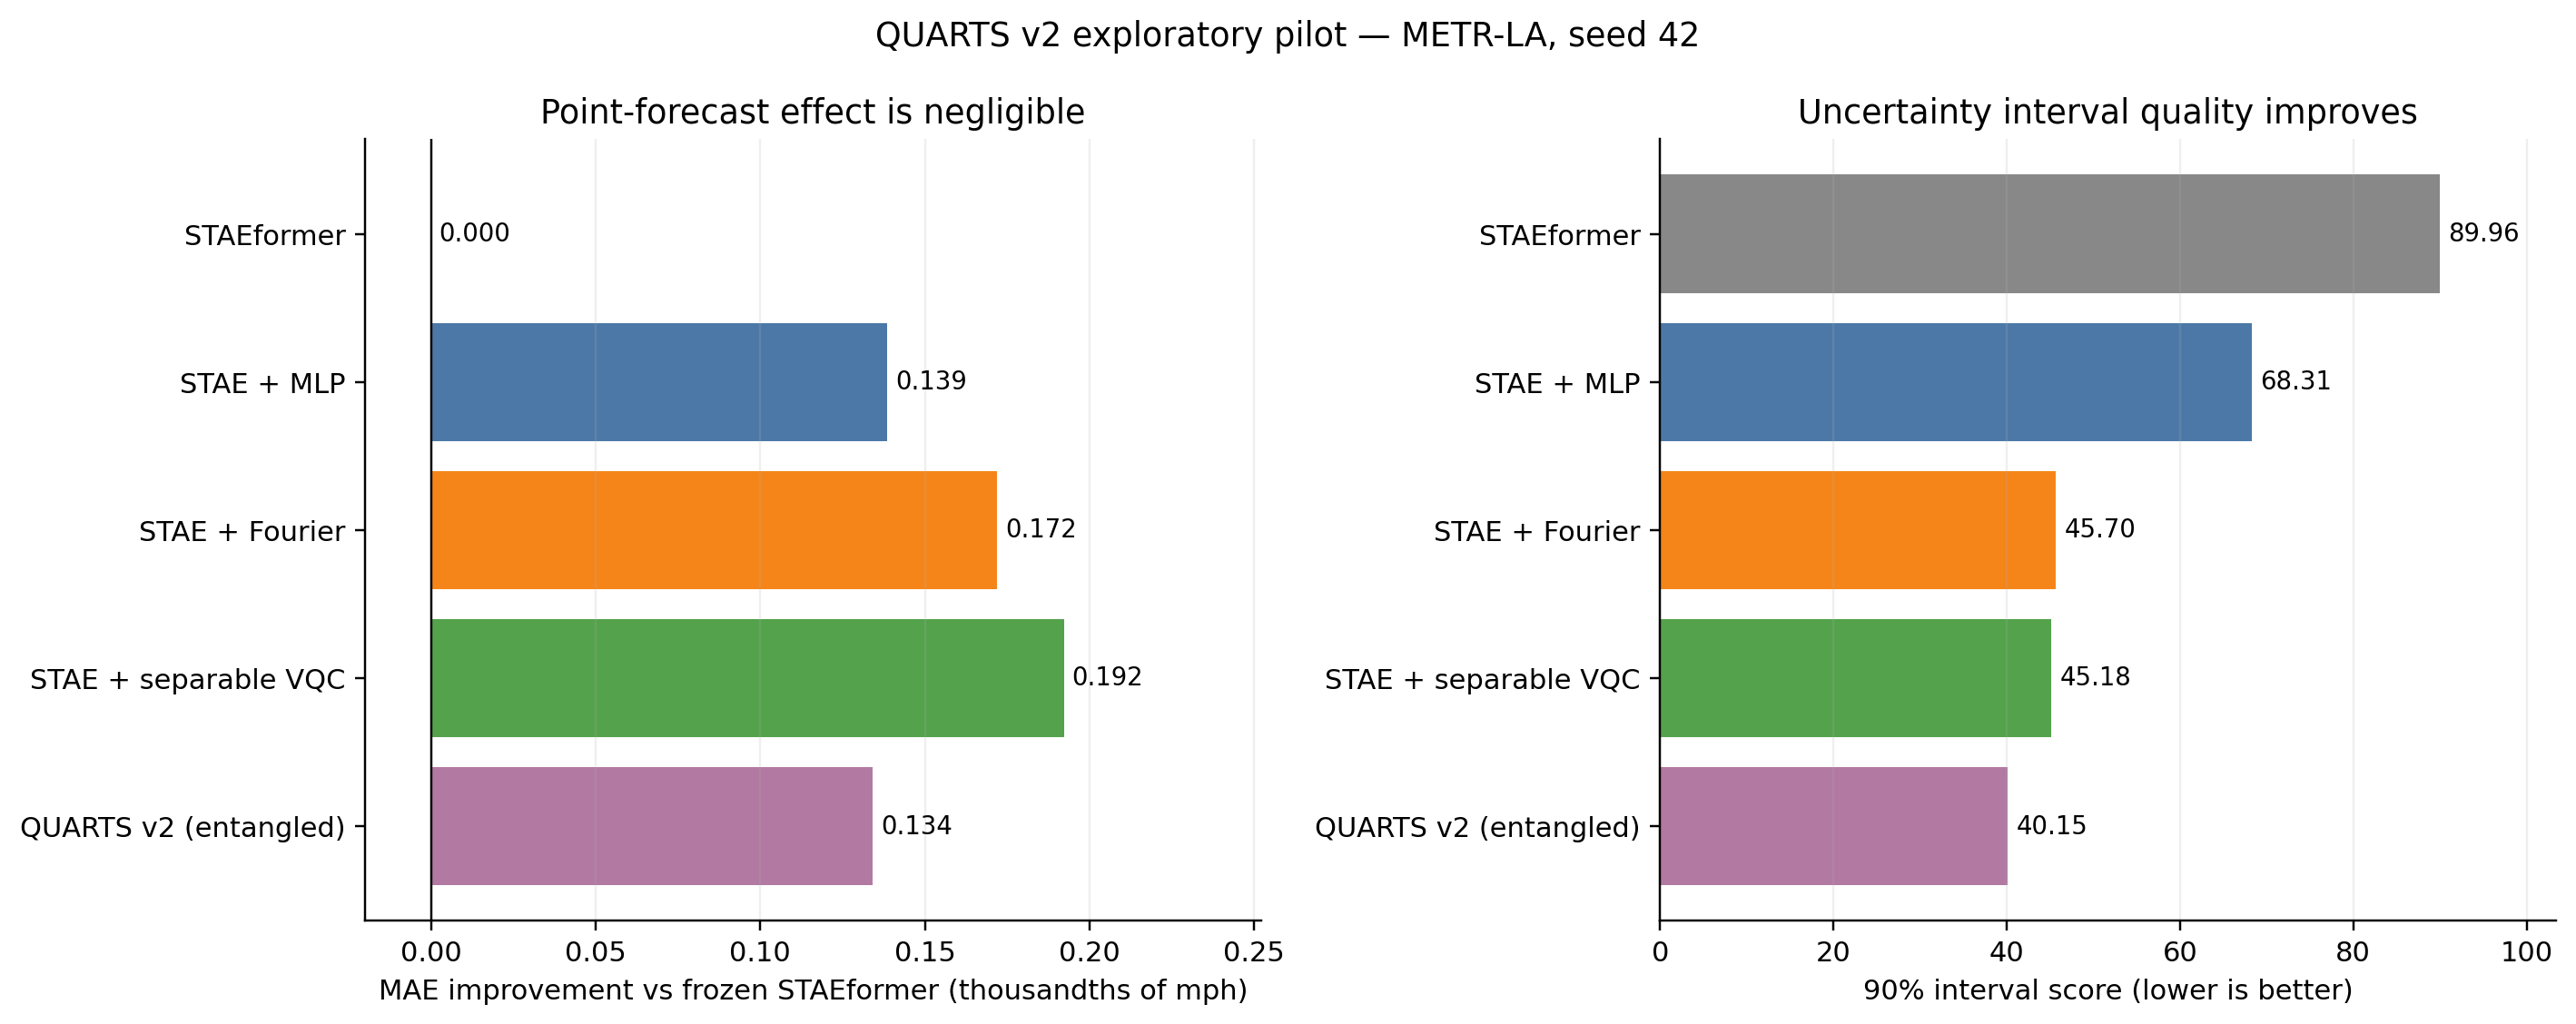
\includegraphics[width=.9\textwidth]{figures/supplement/figureS06_quarts_v2.png}
\caption{QUARTS V2 gated point correction pilot on the validation path. The learned correction remains close to the frozen STAEformer location and does not provide a meaningful point accuracy gain.}
\label{fig:s06}
\end{figure*}

\begin{figure*}[t]
\centering
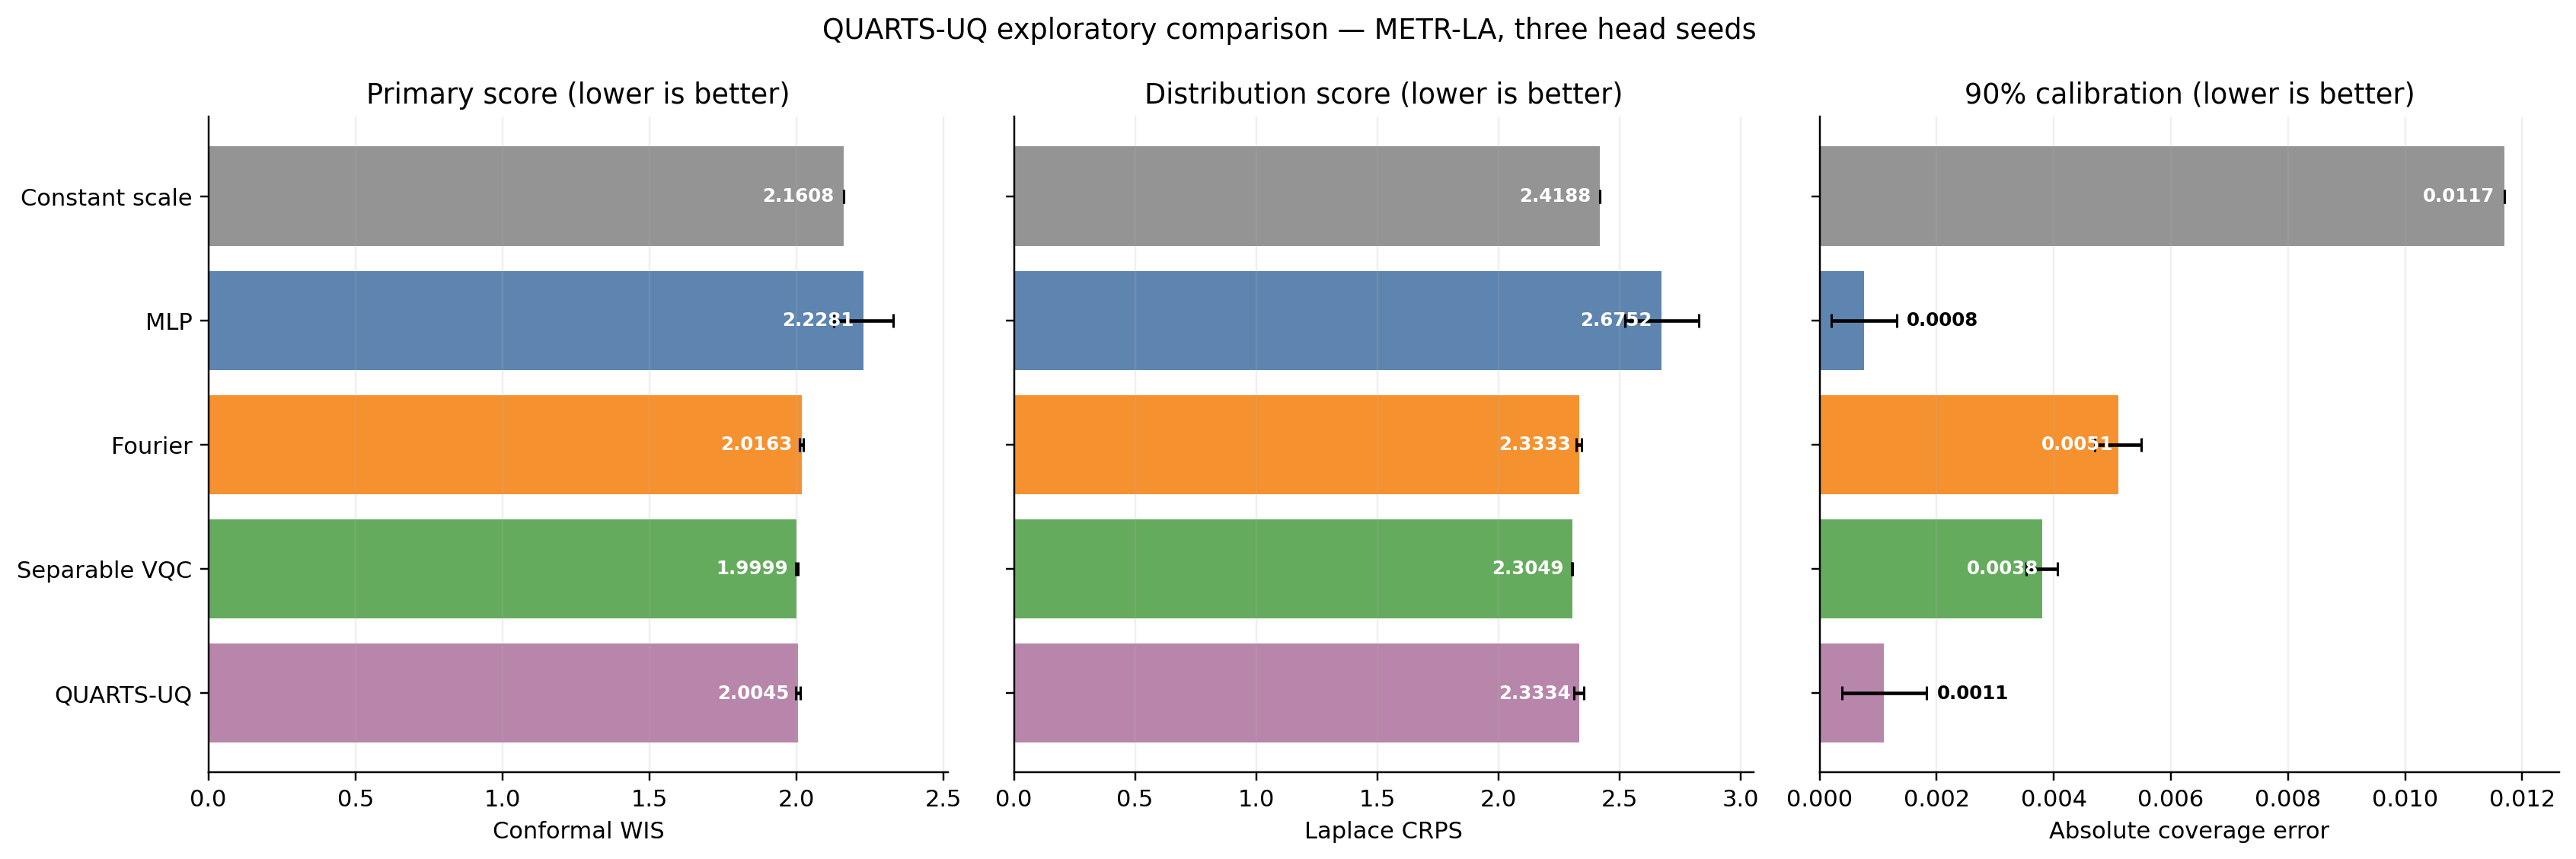
\includegraphics[width=.9\textwidth]{figures/supplement/figureS07_quarts_uq.png}
\caption{QUARTS-UQ uncertainty scale comparison over three head seeds. PASS requires lower WIS than both matched controls and \(90\%\) coverage between \(0.89\) and \(0.91\); the entangled head fails the score requirement.}
\label{fig:s07}
\end{figure*}

\begin{figure*}[t]
\centering
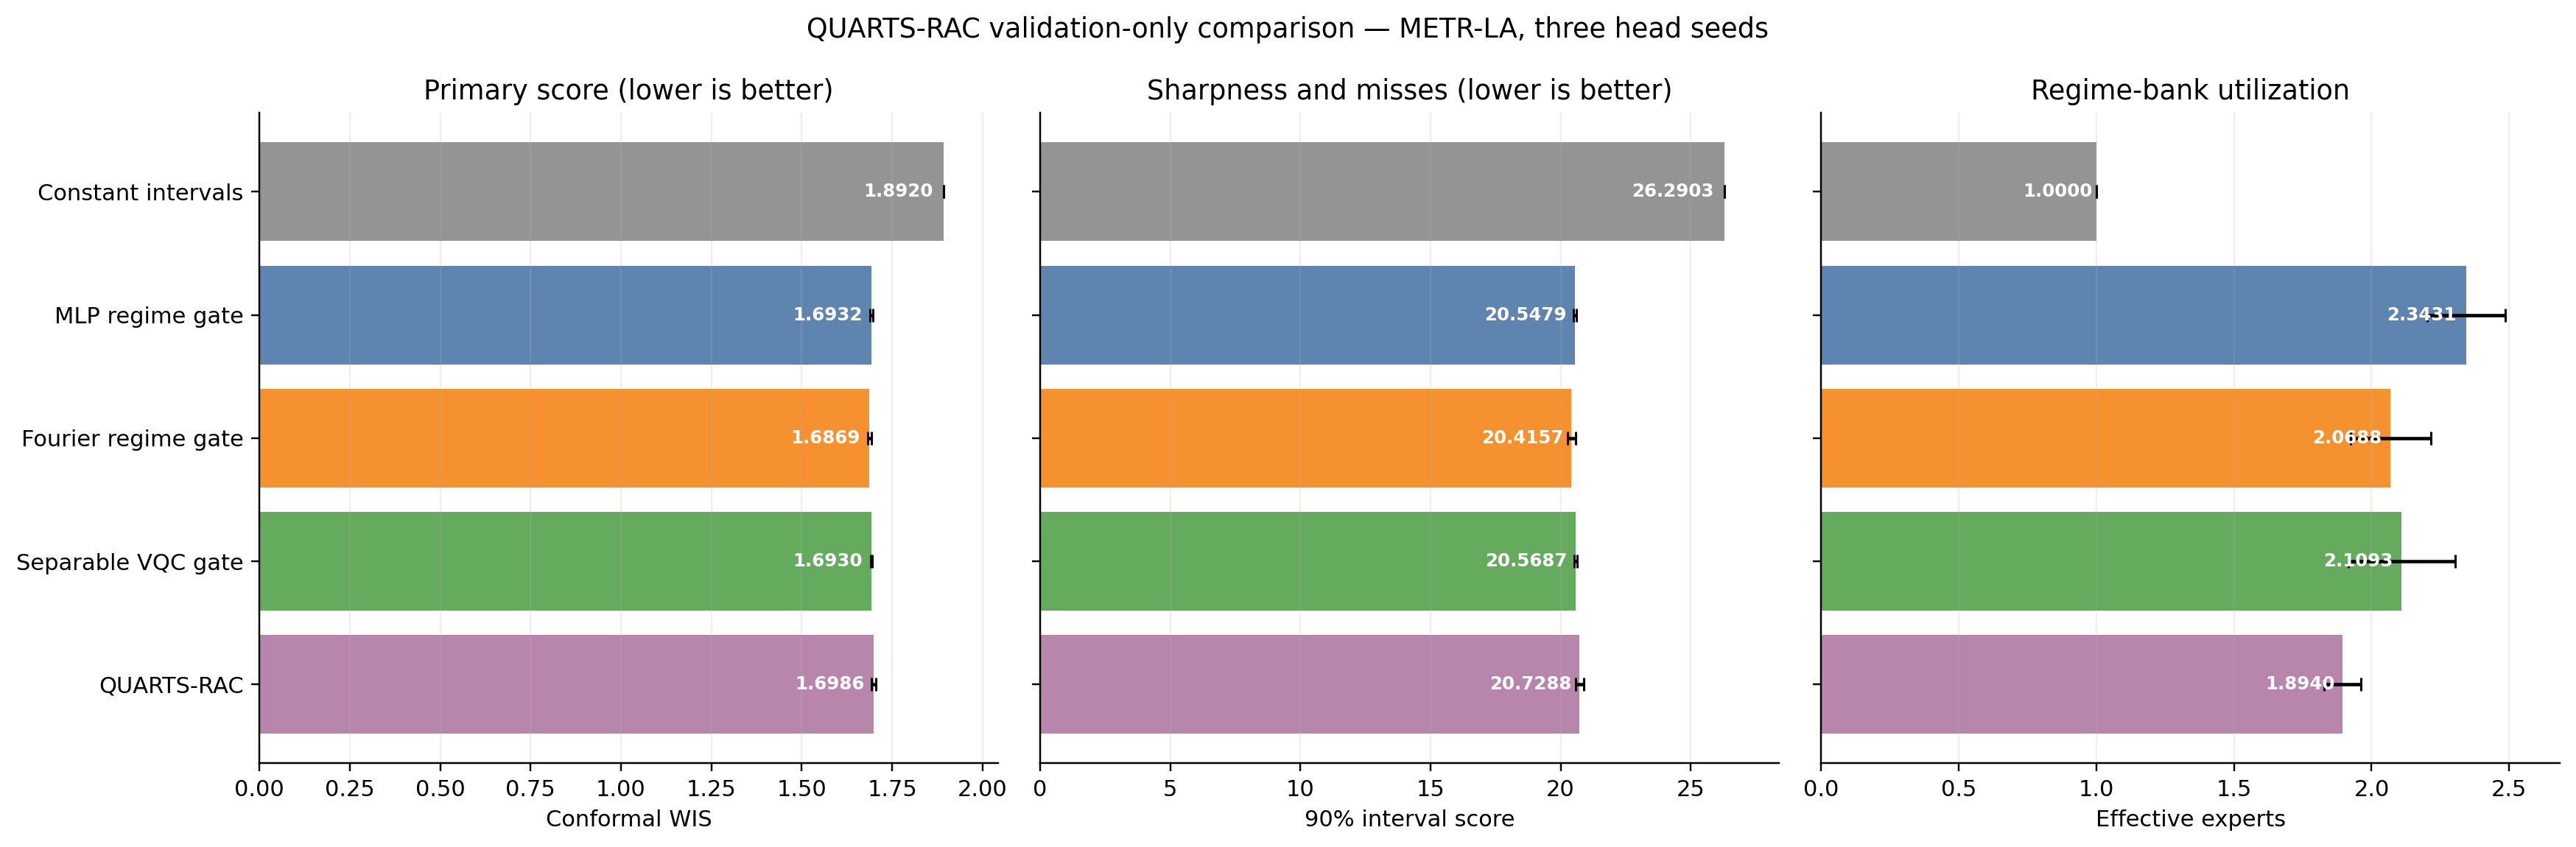
\includegraphics[width=.9\textwidth]{figures/supplement/figureS08_quarts_rac.png}
\caption{Validation only QUARTS-RAC comparison over three head seeds. Fourier-RAC has the lowest mean WIS, while the entangled gate does not pass the required improvement threshold.}
\label{fig:s08}
\end{figure*}

\begin{figure*}[t]
\centering
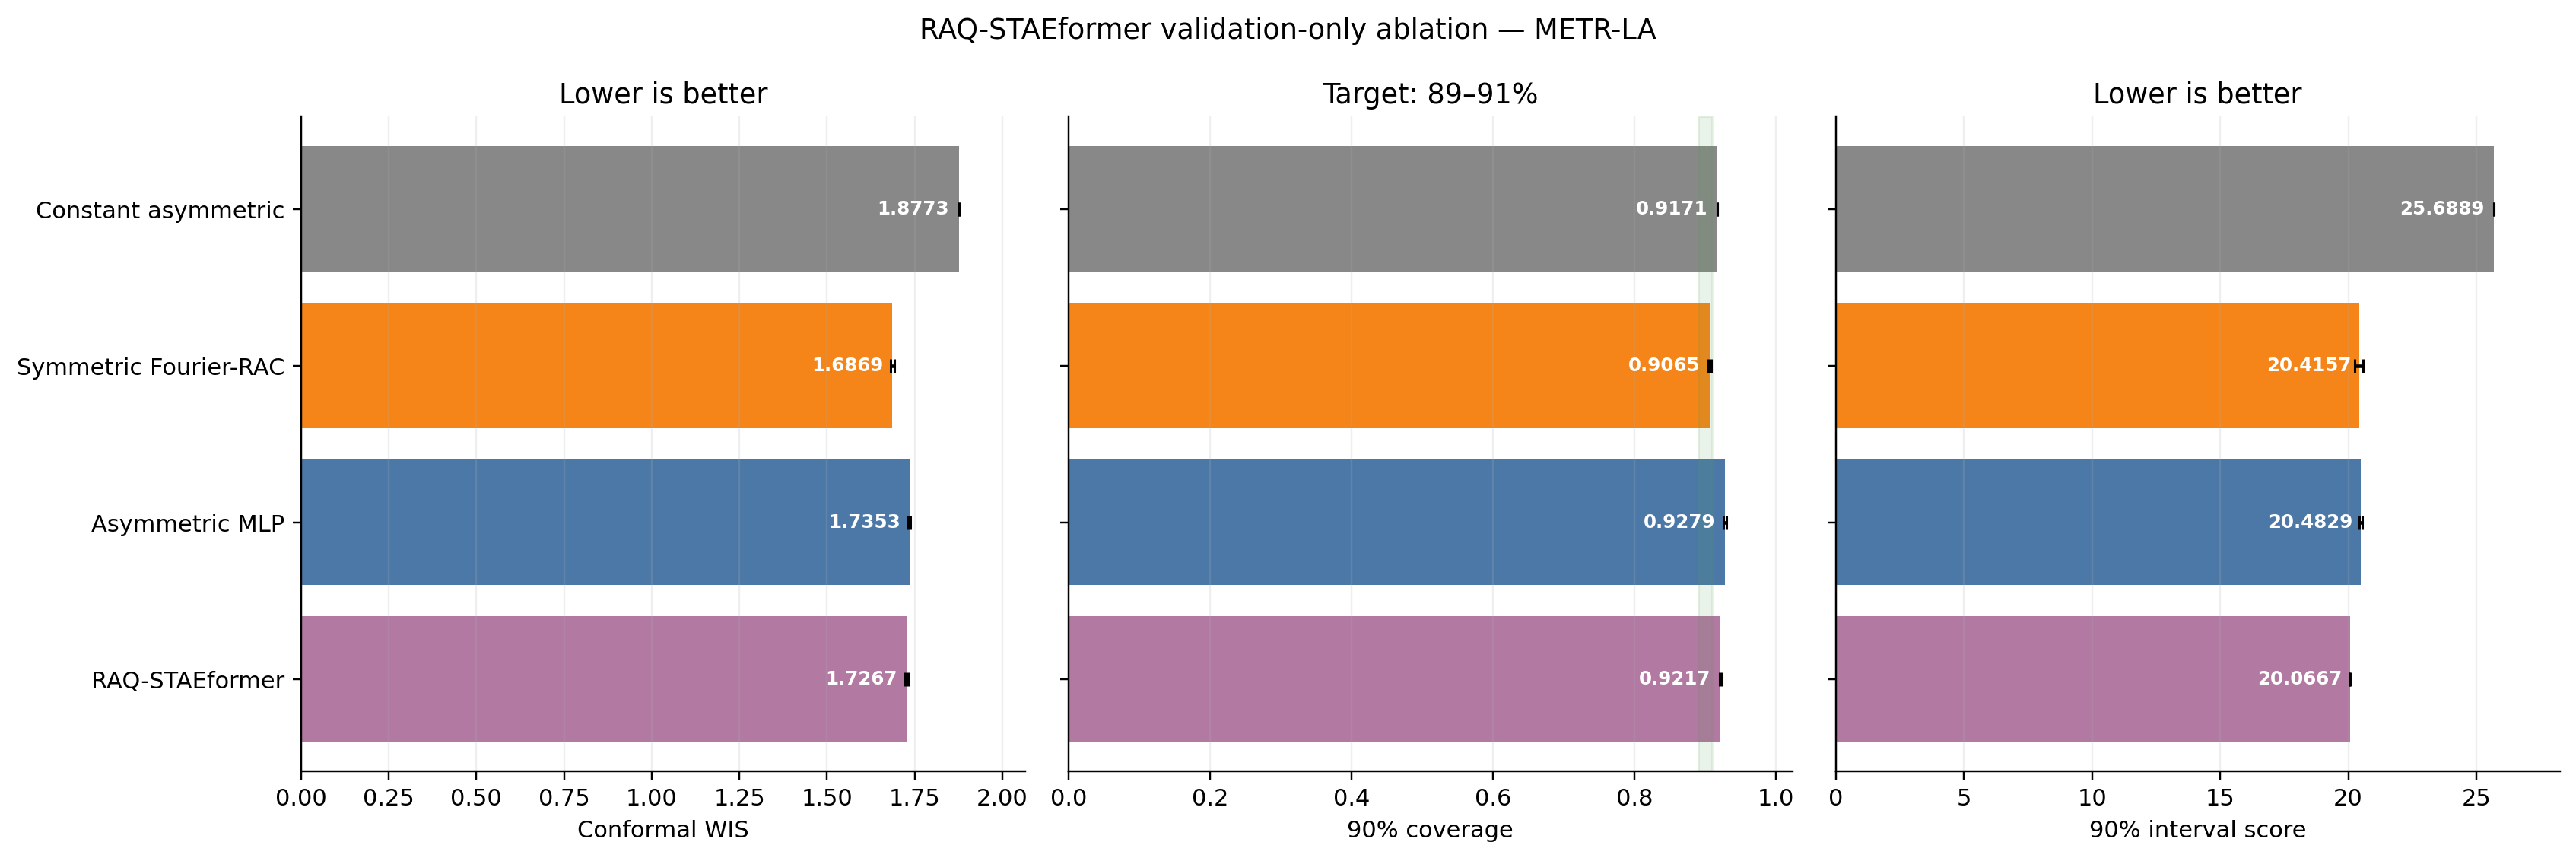
\includegraphics[width=.9\textwidth]{figures/supplement/figureS09_raq_asymmetry.png}
\caption{Asymmetric residual adaptive quantile (RAQ) validation. The asymmetric Fourier head increases WIS and overcovers relative to the symmetric Fourier calibrator, so the branch is not promoted.}
\label{fig:s09}
\end{figure*}

\begin{figure*}[t]
\centering
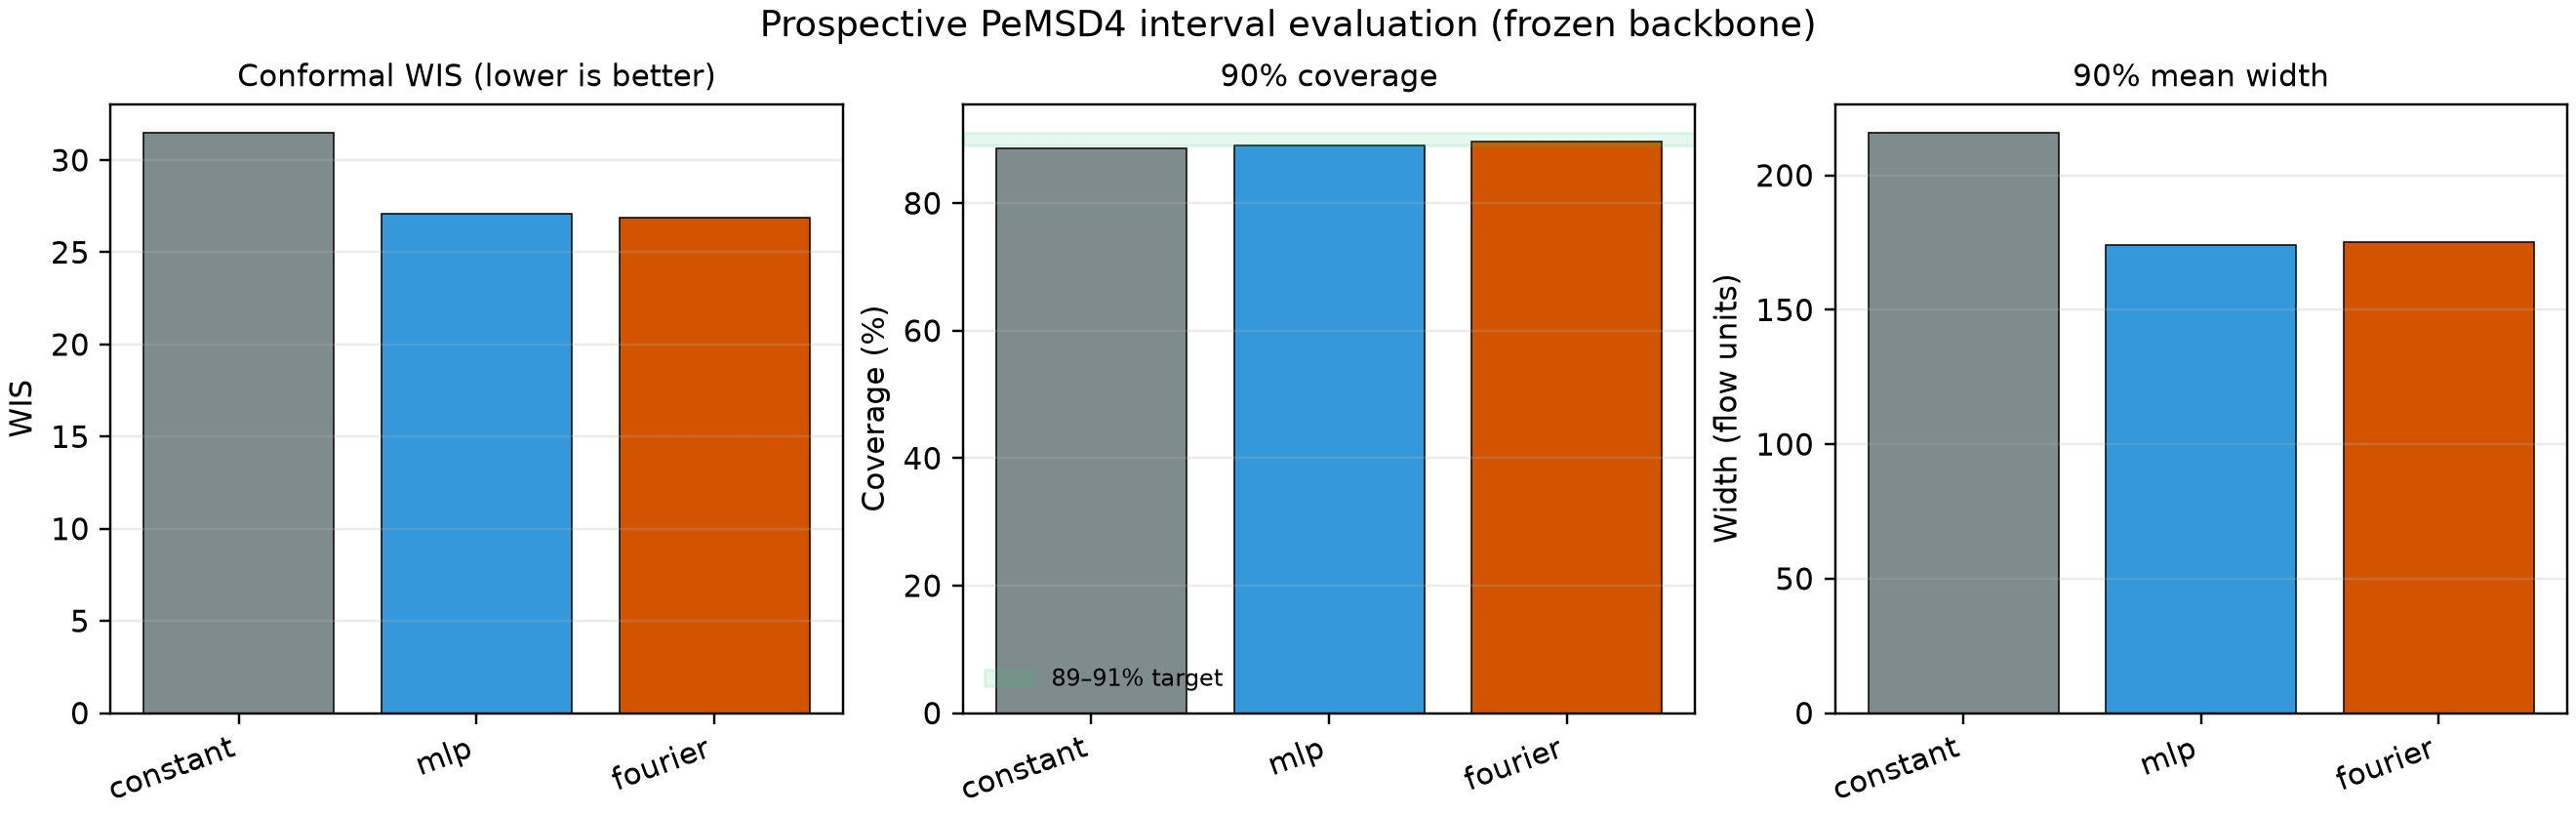
\includegraphics[width=.9\textwidth]{figures/supplement/figureS10_pemsd4_prospective.png}
\caption{Initial prospective PeMSD4 evaluation for backbone seed 42. Fourier-RAC improves WIS relative to constant and MLP intervals while meeting the coverage gate, producing a provisional rather than final pass.}
\label{fig:s10}
\end{figure*}

\begin{figure*}[t]
\centering
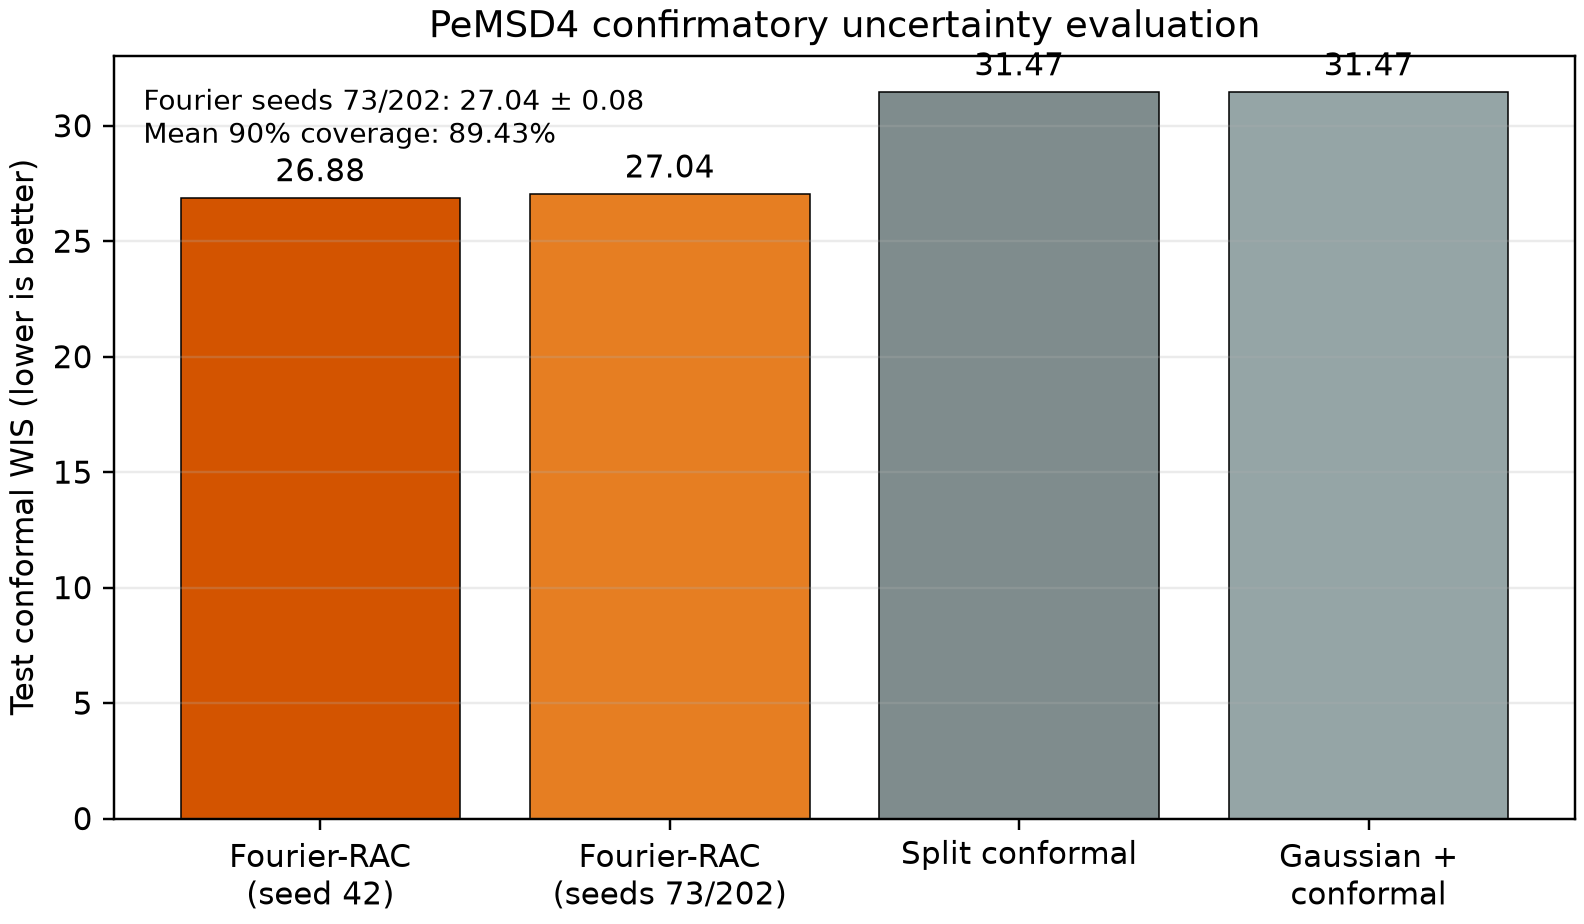
\includegraphics[width=.9\textwidth]{figures/supplement/figureS11_pemsd4_head_seeds.png}
\caption{Original additional PeMSD4 head seed comparison on the seed 42 frozen backbone. Head initialization variation is distinct from the revised five backbone replication, which retrains the complete point model.}
\label{fig:s11}
\end{figure*}

\begin{figure*}[t]
\centering
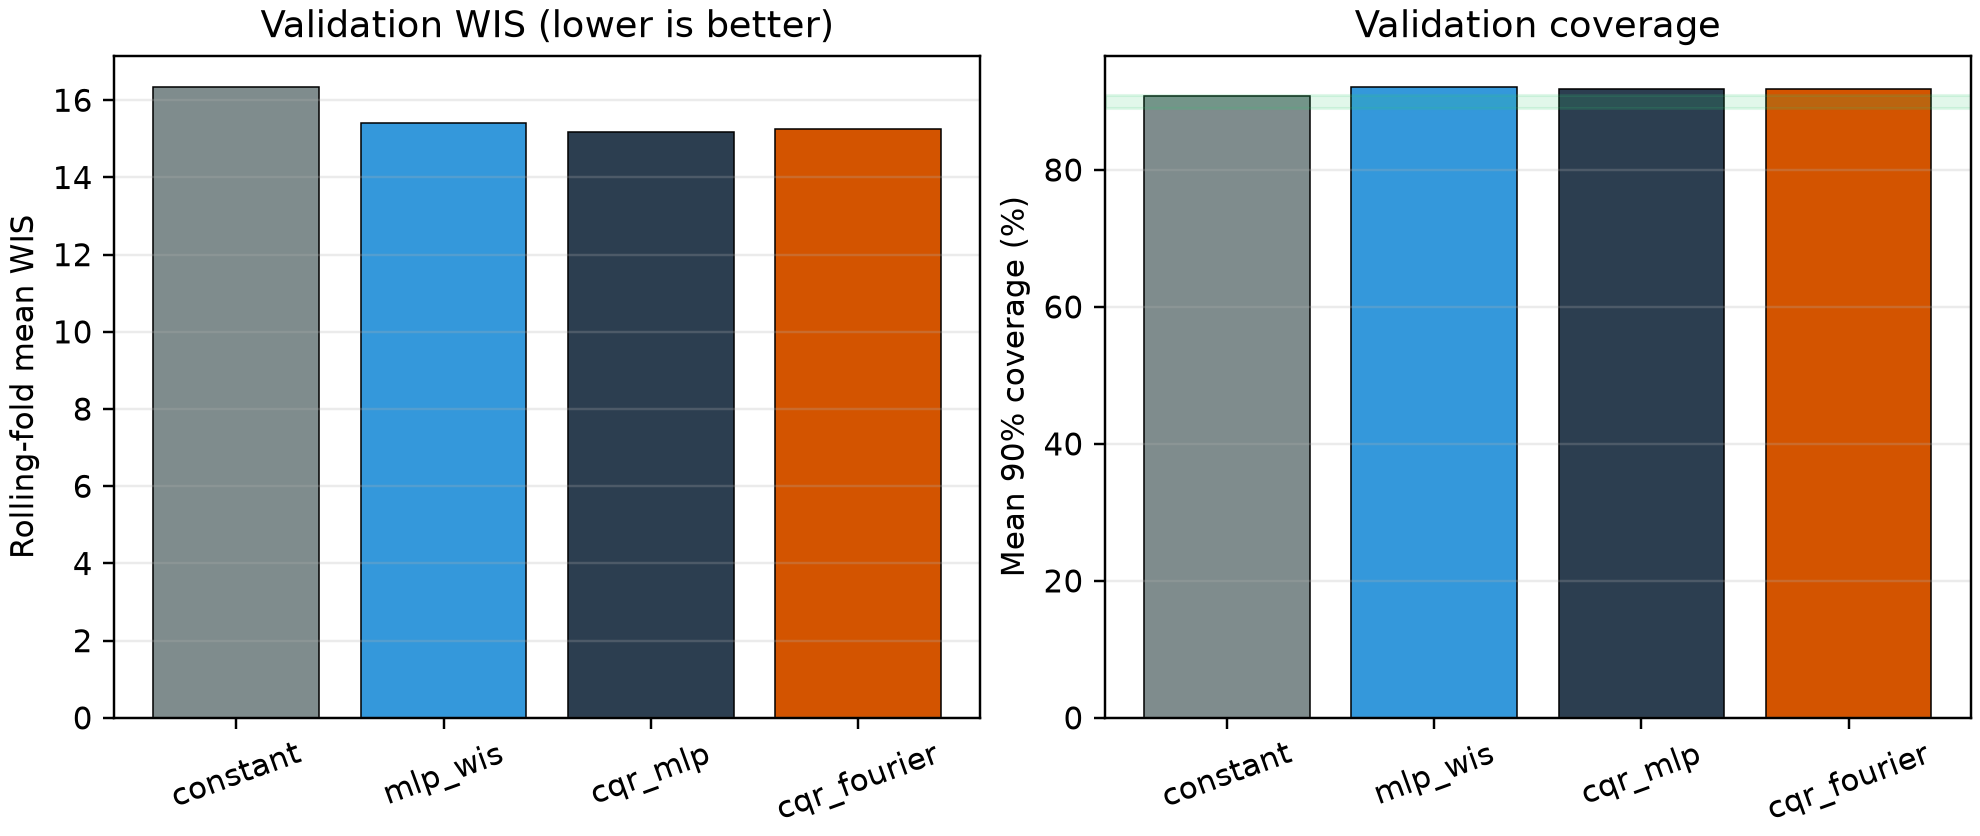
\includegraphics[width=.9\textwidth]{figures/supplement/figureS12_sacqr_validation.png}
\caption{PeMSD8 validation only symmetric adaptive conformal quantile residual (SA-CQR) study over three rolling folds. CQR-Fourier fails its WIS and coverage gate; the canonical PeMSD8 test split remains unused.}
\label{fig:s12}
\end{figure*}

\end{appendices}

\bibliography{references}

\end{document}
